%% The following is a directive for TeXShop to indicate the main file
%%!TEX root = diss.tex

\chapter{Results}
\label{ch:Results}

In this chapter we show results for the BDI cache, the Dedup cache, and the improved implementation caches along with the upper bound we established for DedepBDI. We show how those four cache designs affect compression, MPKI, and speedup.

\section{Methodology}
\label{sec:Methodology}
\begin{table}[]
    \centering
    \begin{tabular}{ll}
        Component & Configuration                                                                                                                                            \\ \hline
        CPU       & x86\_64, 2.6GHz, 4-wide OoO, 80 entry ROB.                                                                                                               \\
        L1I       & 32KB, 4 way, 3 cycle access lat, 64B lines, LRU.                                                                                                         \\
        L1D       & 32KB, 8 way, 4 cycle access lat, 64B lines, LRU.                                                                                                         \\
        L2        & Private, 256KB, 8 way, 11 cycle access lat, 64B lines, LRU.                                                                                              \\
        L3        & \begin{tabular}[c]{@{}l@{}}Shared, 4MB (or similar data array size if compressed),\\  16 way, 39 cycle access lat, 64B lines, 8 banks.\end{tabular} \\
        Mem       & DDR3-1066, 1GB.                                                                                                                                         
        \end{tabular}
    \caption{The simulated system}
    \label{tab:simsys}
\end{table}
\begin{table}[]
    \centering
    \begin{tabular}{|l|l|l|l|}
    \hline
    Compression                   & Cache & Data Entries & Tag Entries \\ \hline
    \multirow{5}{*}{Conventional} & 0.5MB & 8192         & 8192        \\ \cline{2-4} 
                                    & 1MB   & 16384        & 16384       \\ \cline{2-4} 
                                    & 2MB   & 32768        & 32768       \\ \cline{2-4} 
                                    & 4MB   & 65536        & 65536       \\ \cline{2-4} 
                                    & 8MB   & 131072       & 131072      \\ \hline
    \multirow{5}{*}{COMP-2}       & 0.5MB & 8192         & 16384       \\ \cline{2-4} 
                                    & 1MB   & 16384        & 32768       \\ \cline{2-4} 
                                    & 2MB   & 32768        & 65536       \\ \cline{2-4} 
                                    & 4MB   & 65536        & 131072      \\ \cline{2-4} 
                                    & 8MB   & 131072       & 262144      \\ \hline
    \multirow{5}{*}{COMP-4}       & 0.5MB & 8192         & 32768       \\ \cline{2-4} 
                                    & 1MB   & 16384        & 65536       \\ \cline{2-4} 
                                    & 2MB   & 32768        & 131072      \\ \cline{2-4} 
                                    & 4MB   & 65536        & 262144      \\ \cline{2-4} 
                                    & 8MB   & 131072       & 524288      \\ \cline{2-4} 
    \end{tabular}
    \caption{All cache configurations.}
    \label{tab:simcache}
\end{table}
We used the zsim~\cite{zsim} simulator to design and implement the four target caches: BDI, Dedup, DedupBDI, and Ideal DedupBDI along with a baseline conventional (uncompressed) cache. We used an out-of-order core timing model based on a medium-size x86 core, with detailed timing for all critical-path and off-critical-path events. We simulated a system with a 3 level cache hierarchy, with private L1 and L2 caches and a shared L3 cache. The simulated system is listed in Table~\ref{tab:simsys}.\par 
We simulated different conventional L3 cache sizes ranging from 0.5MB to 8MB. We also simulated the four compressed caches at the same data array sizes, but with tag arrays double and four times of the data lines. For example, a 4MB-2 BDI cache has the same data array as a conventional 4MB cache, but its tag to data ratio is 2 so its tag array size is double its conventional counterpart. The LLC cache configurations are shown in~\ref{tab:simcache}. The workloads used are all the benchmarks from the AxBench~\cite{axbench} benchmark suite, the Parsec~\cite{parsec} benchmark suite with simmedium inputs, and the Spec~\cite{spec} benchmark suite with train inputs (mid-size inputs). All the benchmarks were simulated until end or 3 billion instructions.\par
The offline analysis done in Chapters~\ref{ch:BackgroundMotiv} and~\ref{ch:Design} were done using a modified version of zsim. zsim was used to dump cache contents every 100,000 L3 accesses, then the dumps were used for data line pattern analysis.

\section{Case Study}
\label{sec:case_study}
In this section we describe the four benchmarks we picked in~\ref{sec:Motivation}. The benchmarks have different cache patterns and behaviors. Recall that during the offline cache dump analysis done in~\ref{sec:Motivation} canneal was only compressible by BDI, dedup was compressible using deduplication, jmeint was incompressible, and libquantum was compressible by both. We analyze how these benchmarks behave when simulated in a real computing system with compressed caches.\par
\begin{figure}
    \begin{subfigure}{\textwidth}
        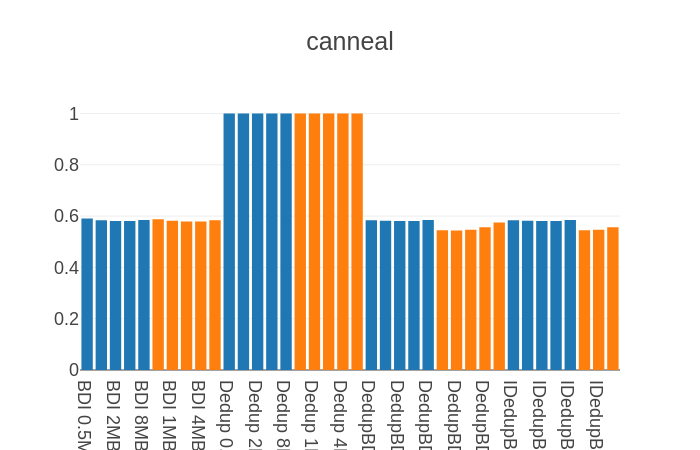
\includegraphics[width=\textwidth]{canneal-compratio.png}
        \caption{canneal}
    \end{subfigure}
    \begin{subfigure}{\textwidth}
        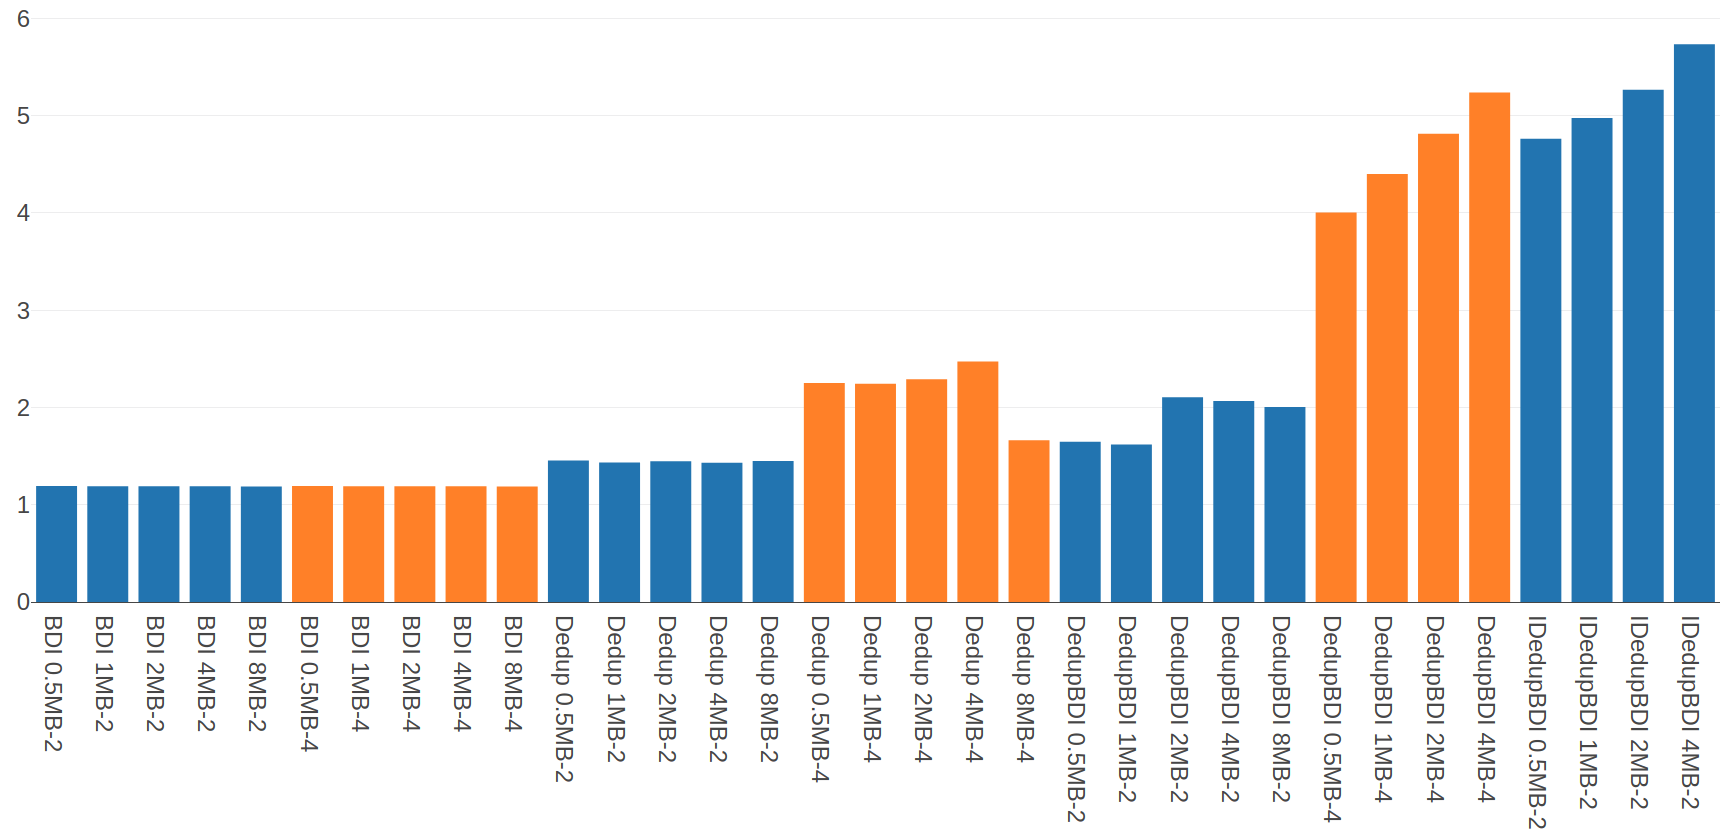
\includegraphics[width=\textwidth]{lbm-compratio.png}
        \caption{lbm}
    \end{subfigure}
    \caption[Case Study: Compression1]{Showing four benchmarks and their compression ratio using different compressed caches.}
    \label{fig:case_compratio1}
\end{figure}
\begin{figure}
    \begin{subfigure}{\textwidth}
        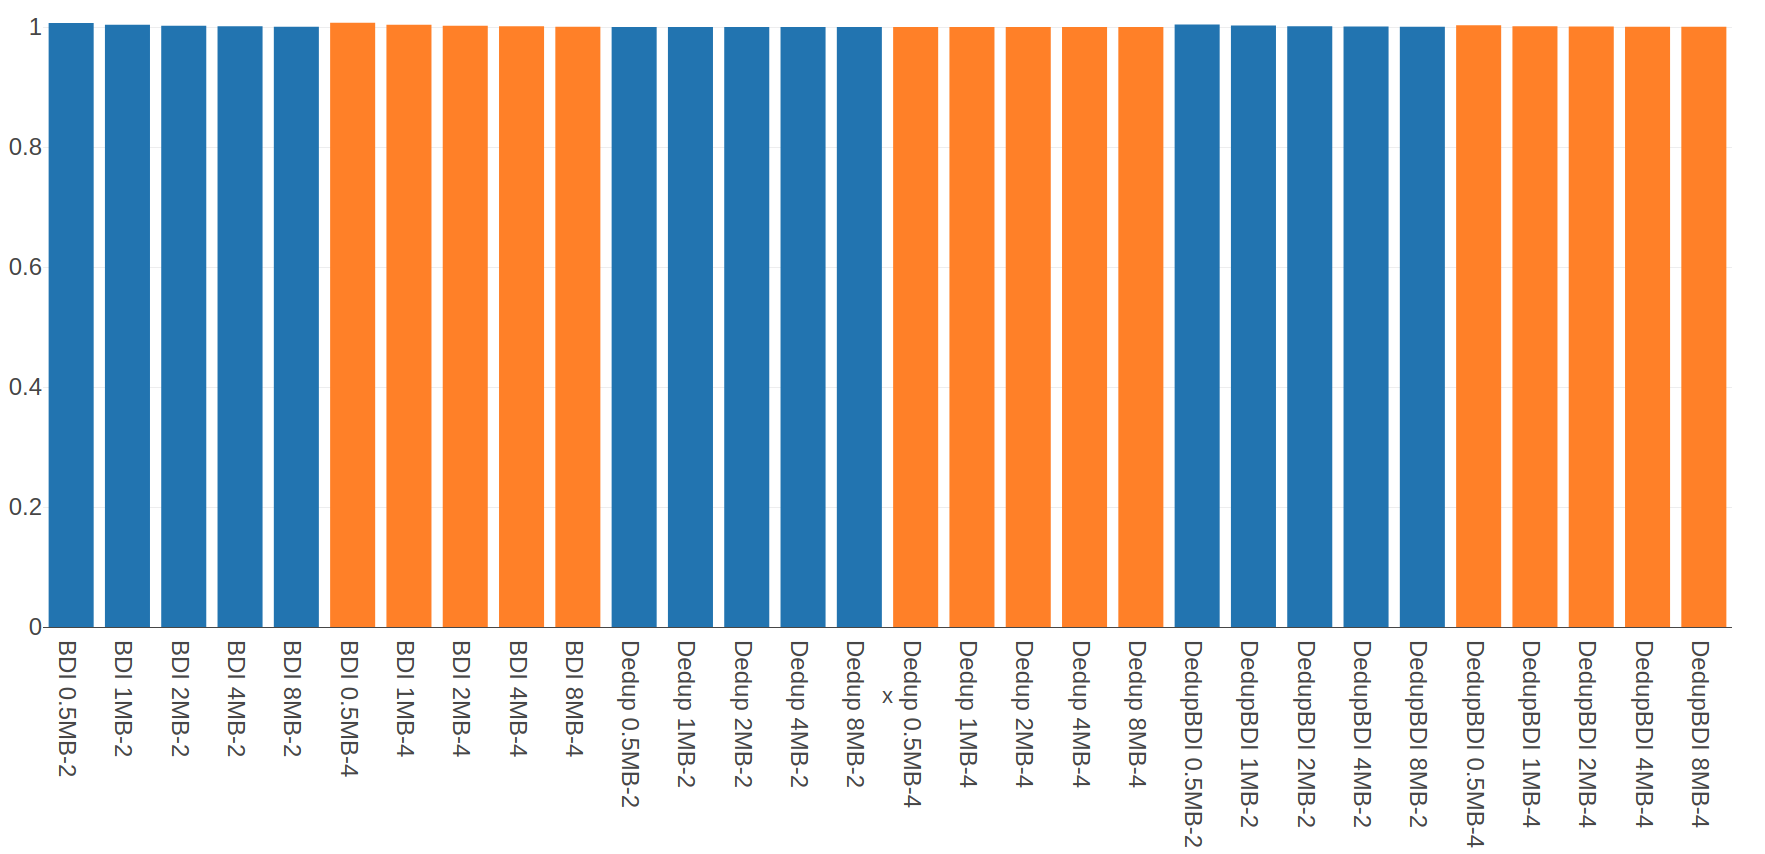
\includegraphics[width=\textwidth]{jmeint-compratio.png}
        \caption{jmeint}
    \end{subfigure}
    \begin{subfigure}{\textwidth}
        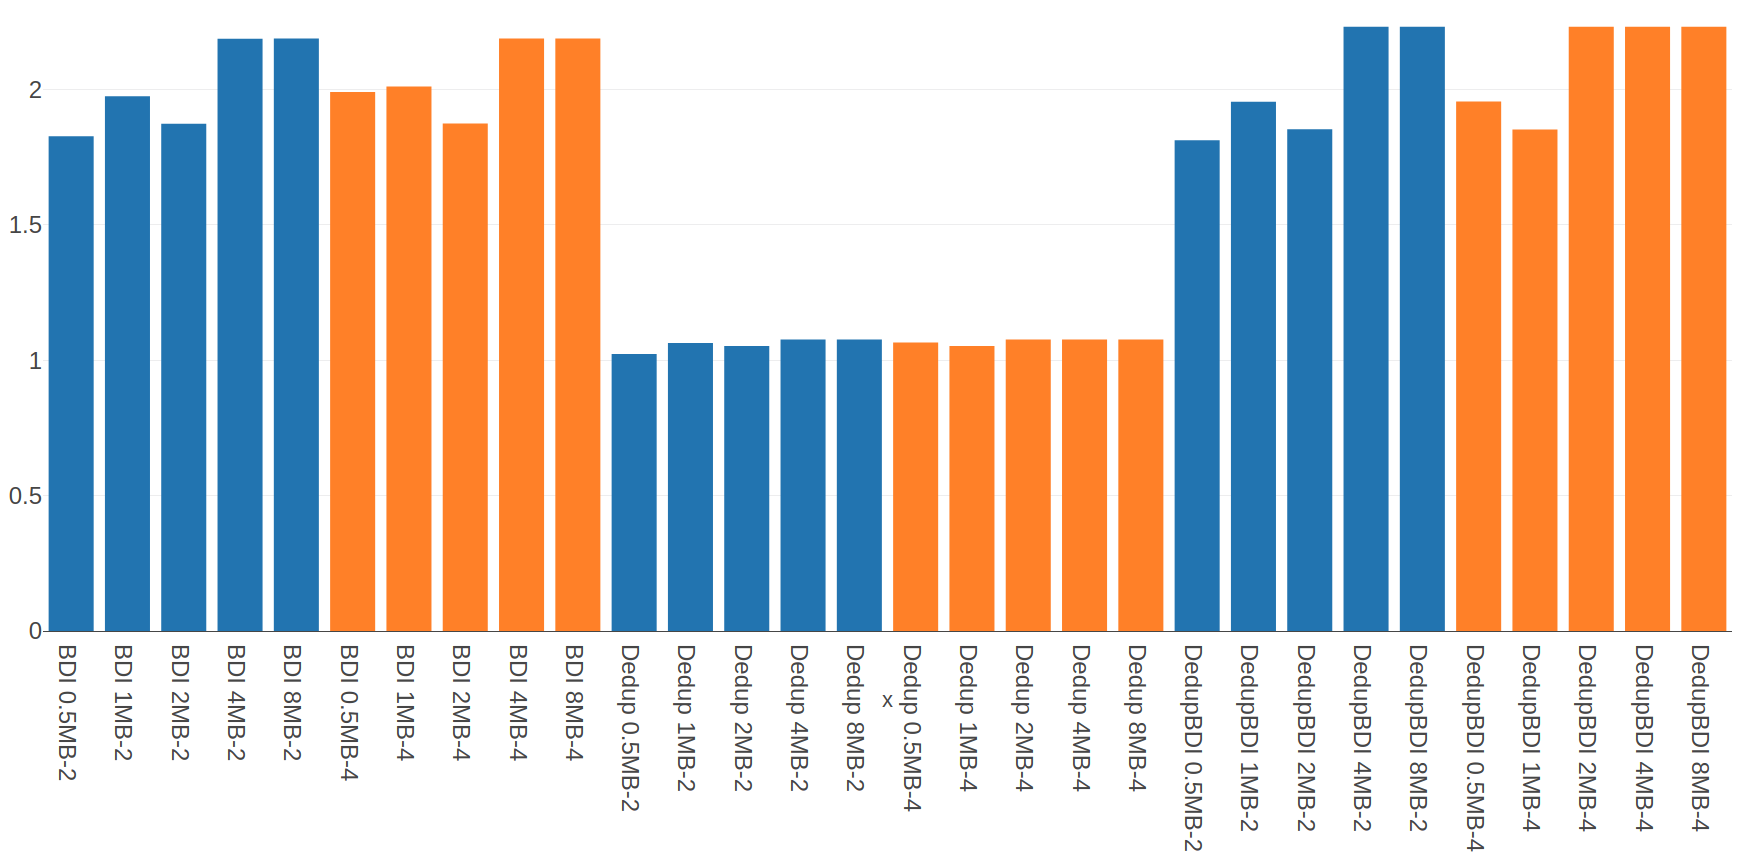
\includegraphics[width=\textwidth]{libquantum-compratio.png}
        \caption{libquantum}
    \end{subfigure}
    \caption[Case Study: Compression2]{Showing four benchmarks and their compression ratio using different compressed caches.}
    \label{fig:case_compratio2}
\end{figure}
\begin{figure}
    \begin{subfigure}{0.5\textwidth}
        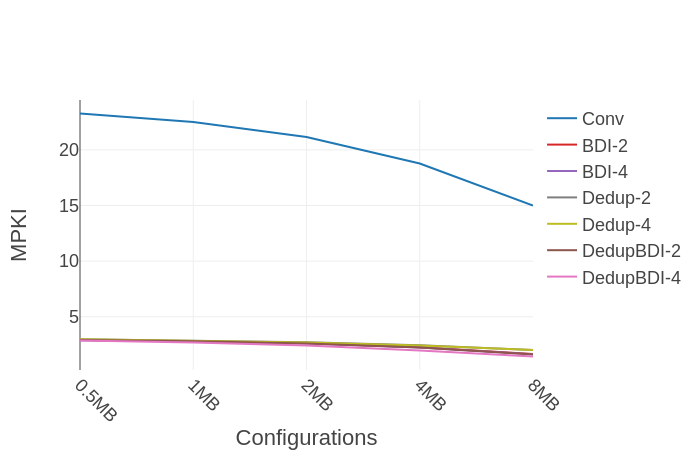
\includegraphics[width=\textwidth]{canneal-mpki.png}
        \caption{canneal}
    \end{subfigure}
    \begin{subfigure}{0.5\textwidth}
        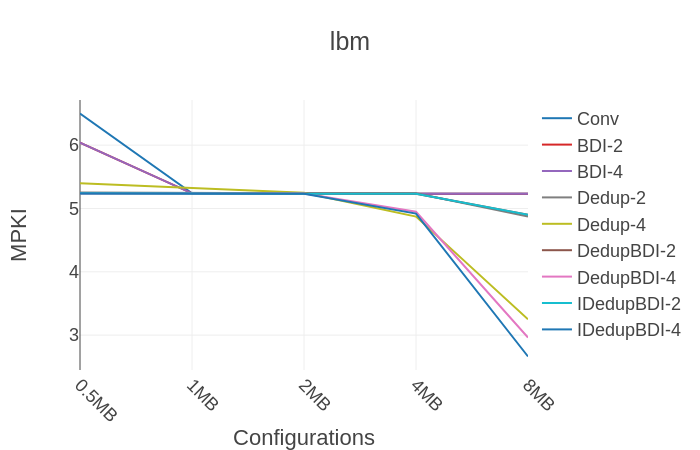
\includegraphics[width=\textwidth]{lbm-mpki.png}
        \caption{lbm}
    \end{subfigure}
    \begin{subfigure}{0.5\textwidth}
        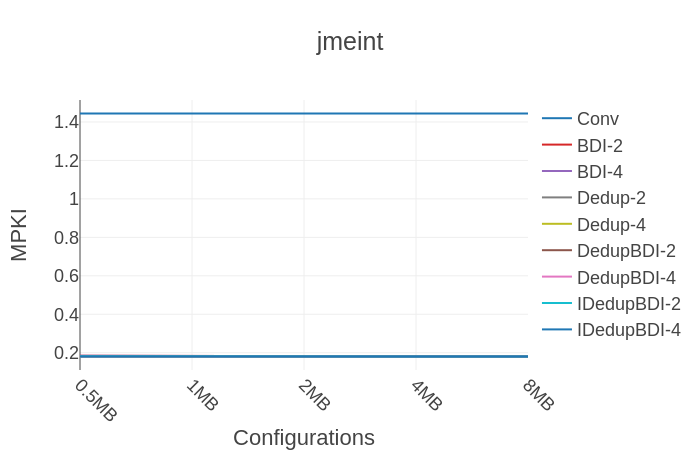
\includegraphics[width=\textwidth]{jmeint-mpki.png}
        \caption{jmeint}
    \end{subfigure}
    \begin{subfigure}{0.5\textwidth}
        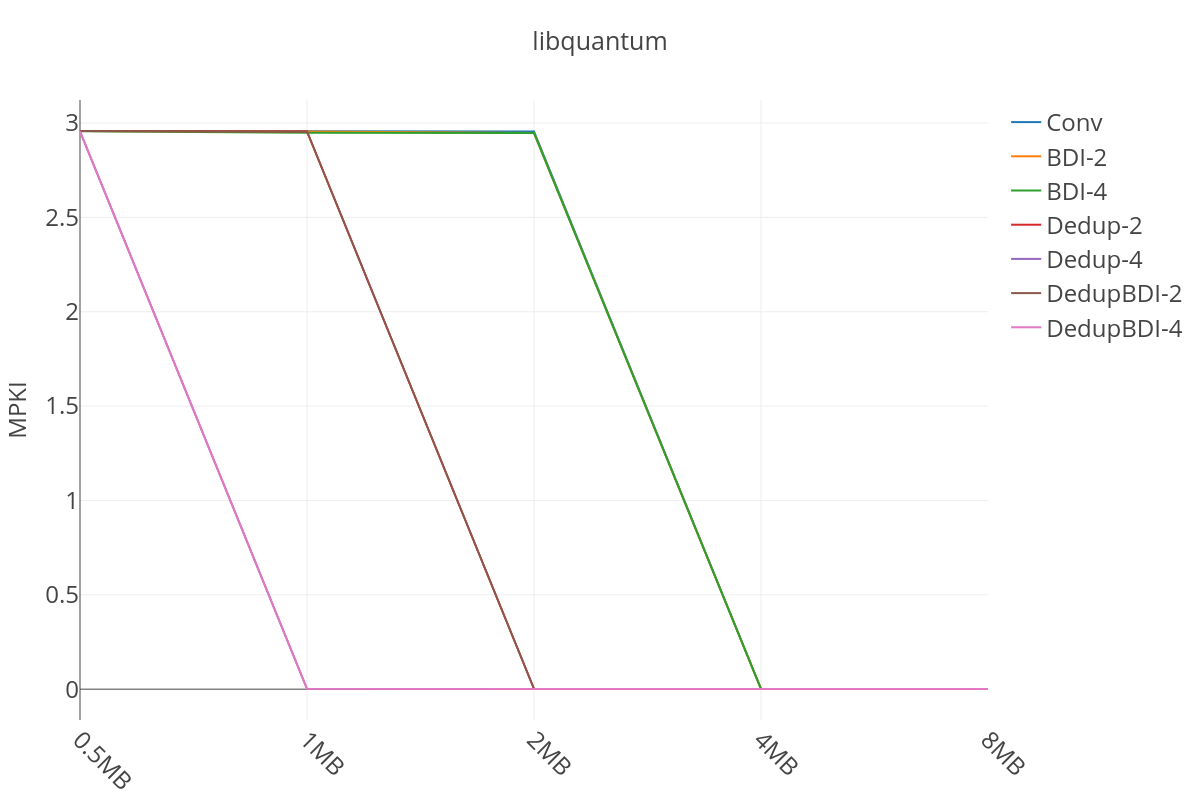
\includegraphics[width=\textwidth]{libquantum-mpki.png}
        \caption{libquantum}
    \end{subfigure}
    \caption[Case Study: MPKI]{Showing four benchmarks and their MPKI using different compressed caches.}
    \label{fig:case_mpki}
\end{figure}
\begin{figure}
    \begin{subfigure}{0.5\textwidth}
        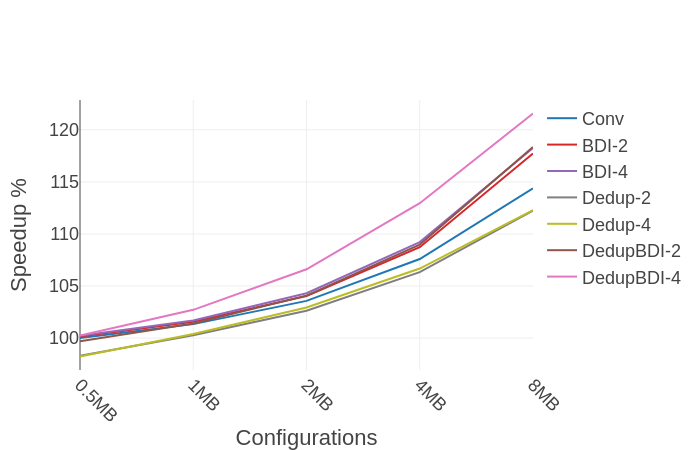
\includegraphics[width=\textwidth]{canneal-speedup.png}
        \caption{canneal}
    \end{subfigure}
    \begin{subfigure}{0.5\textwidth}
        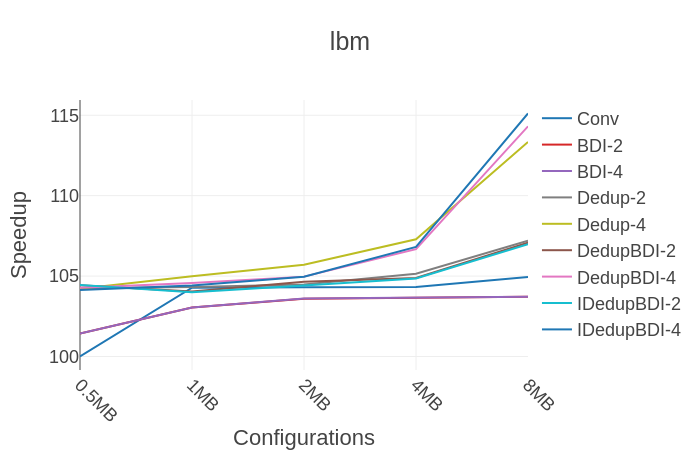
\includegraphics[width=\textwidth]{lbm-speedup.png}
        \caption{lbm}
    \end{subfigure}
    \begin{subfigure}{0.5\textwidth}
        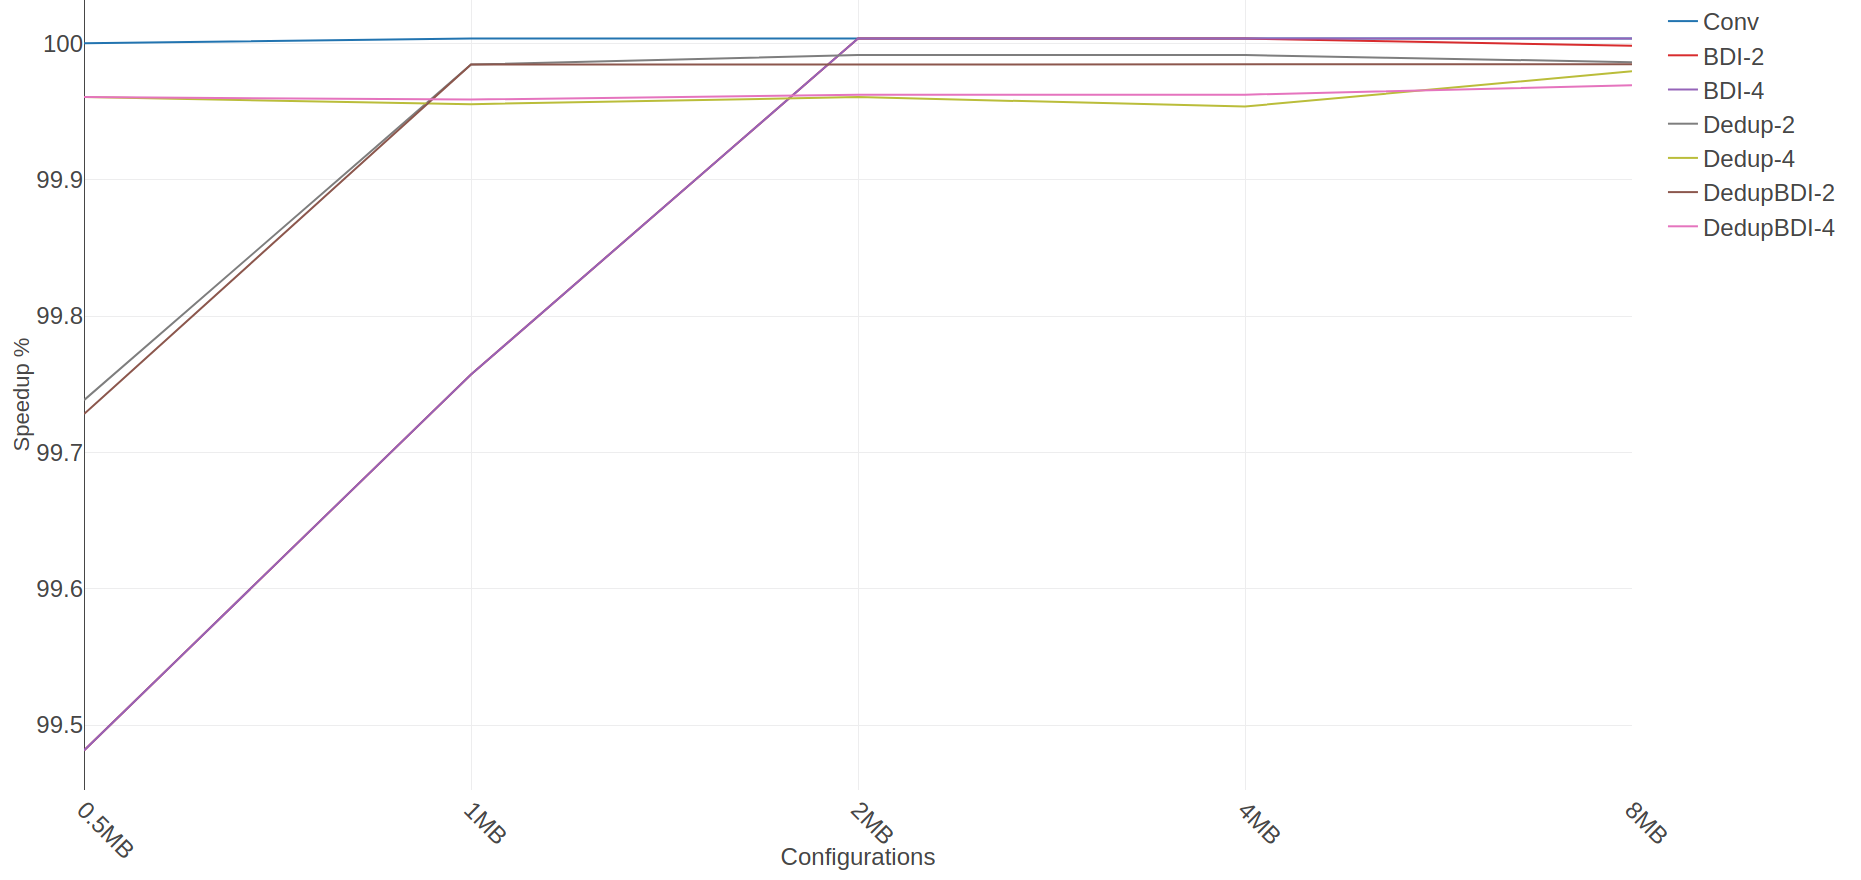
\includegraphics[width=\textwidth]{jmeint-speedup.png}
        \caption{jmeint}
    \end{subfigure}
    \begin{subfigure}{0.5\textwidth}
        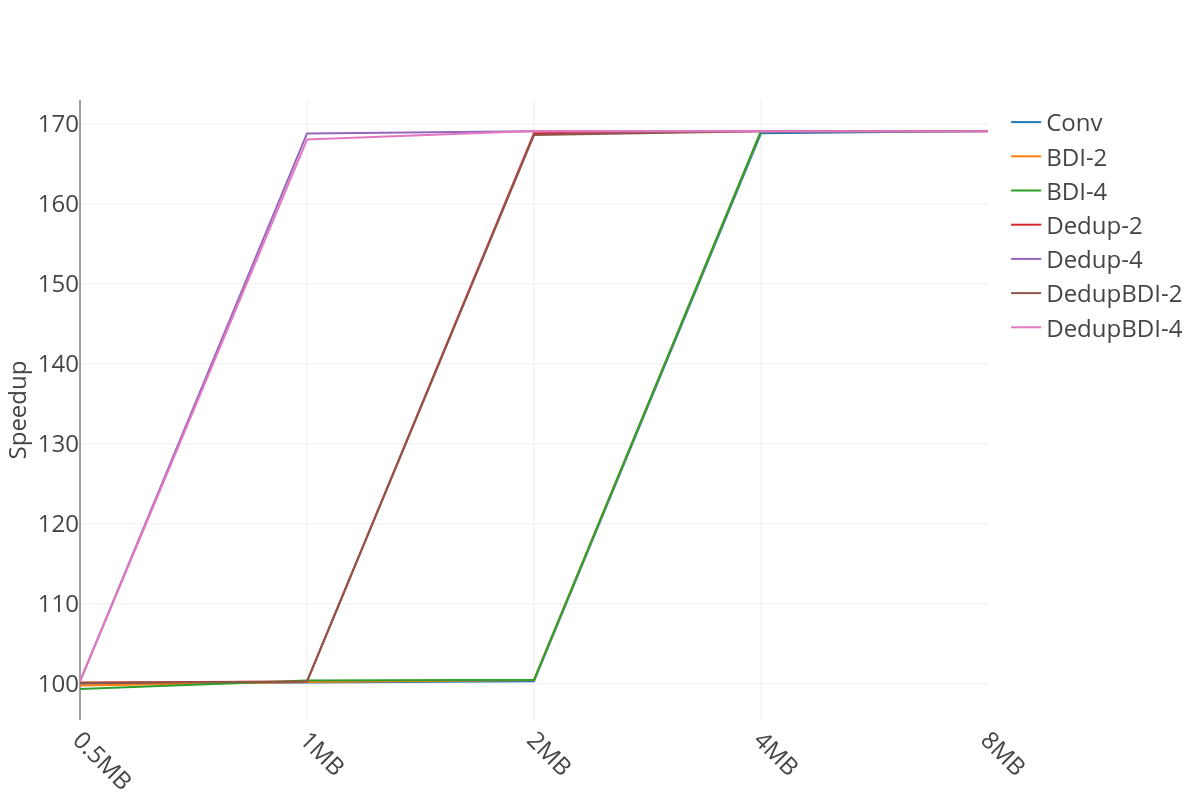
\includegraphics[width=\textwidth]{libquantum-speedup.png}
        \caption{libquantum}
    \end{subfigure}
    \caption[Case Study: Speedup]{Showing four benchmarks and their speedup using different compressed caches.}
    \label{fig:case_speedup}
\end{figure}
Figures~\ref{fig:case_compratio1} and~\ref{fig:case_compratio2} show the compression ratio of the four benchmarks. Compression ratio is calculated as the ratio between valid tags and valid data entries. The blue columns are caches with tag entries double the data entries, while the orange ones have tags four times the data entries. As expected, canneal shows some compression with BDI but nothing with Dedup, lbm shows compression using Dedup but not using BDI, jmeint shows no compression using any of the caches, while libquantum shows compression using all of them. The DedupBDI cache combines both compressions and either outperforms or at least does as well as BDI or Dedup.\par
Figures~\ref{fig:case_mpki} and~\ref{fig:case_speedup} show the MPKI and Speedup for the four benchmarks under all cache configurations. Apart from the incompressible jmeint, all the benchmarks show big speedups (up to 70\% in case of libquantum). DedupBDI is the best performing cache in canneal, lbm and libquantum. But it is slightly worse (0.05\% slowdown) than a conventional cache in jmeint.\par
The results shown are in sync with the offline analysis we did in section~\ref{sec:Motivation}. This shows how the DedupBDI cache brings together the best of both worlds. It is able to function exactly similar to BDI and Dedup in cases that are only compressible by one, and it is able to use both compressions at the same time to enhance compression and performance. Rhe cost for this is its increased complexity and access latency that causes it to perform slightly worse in incompressible cases.

\section{Compression}
\label{sec:Compression}
\begin{figure}
    \begin{subfigure}{\textwidth}
        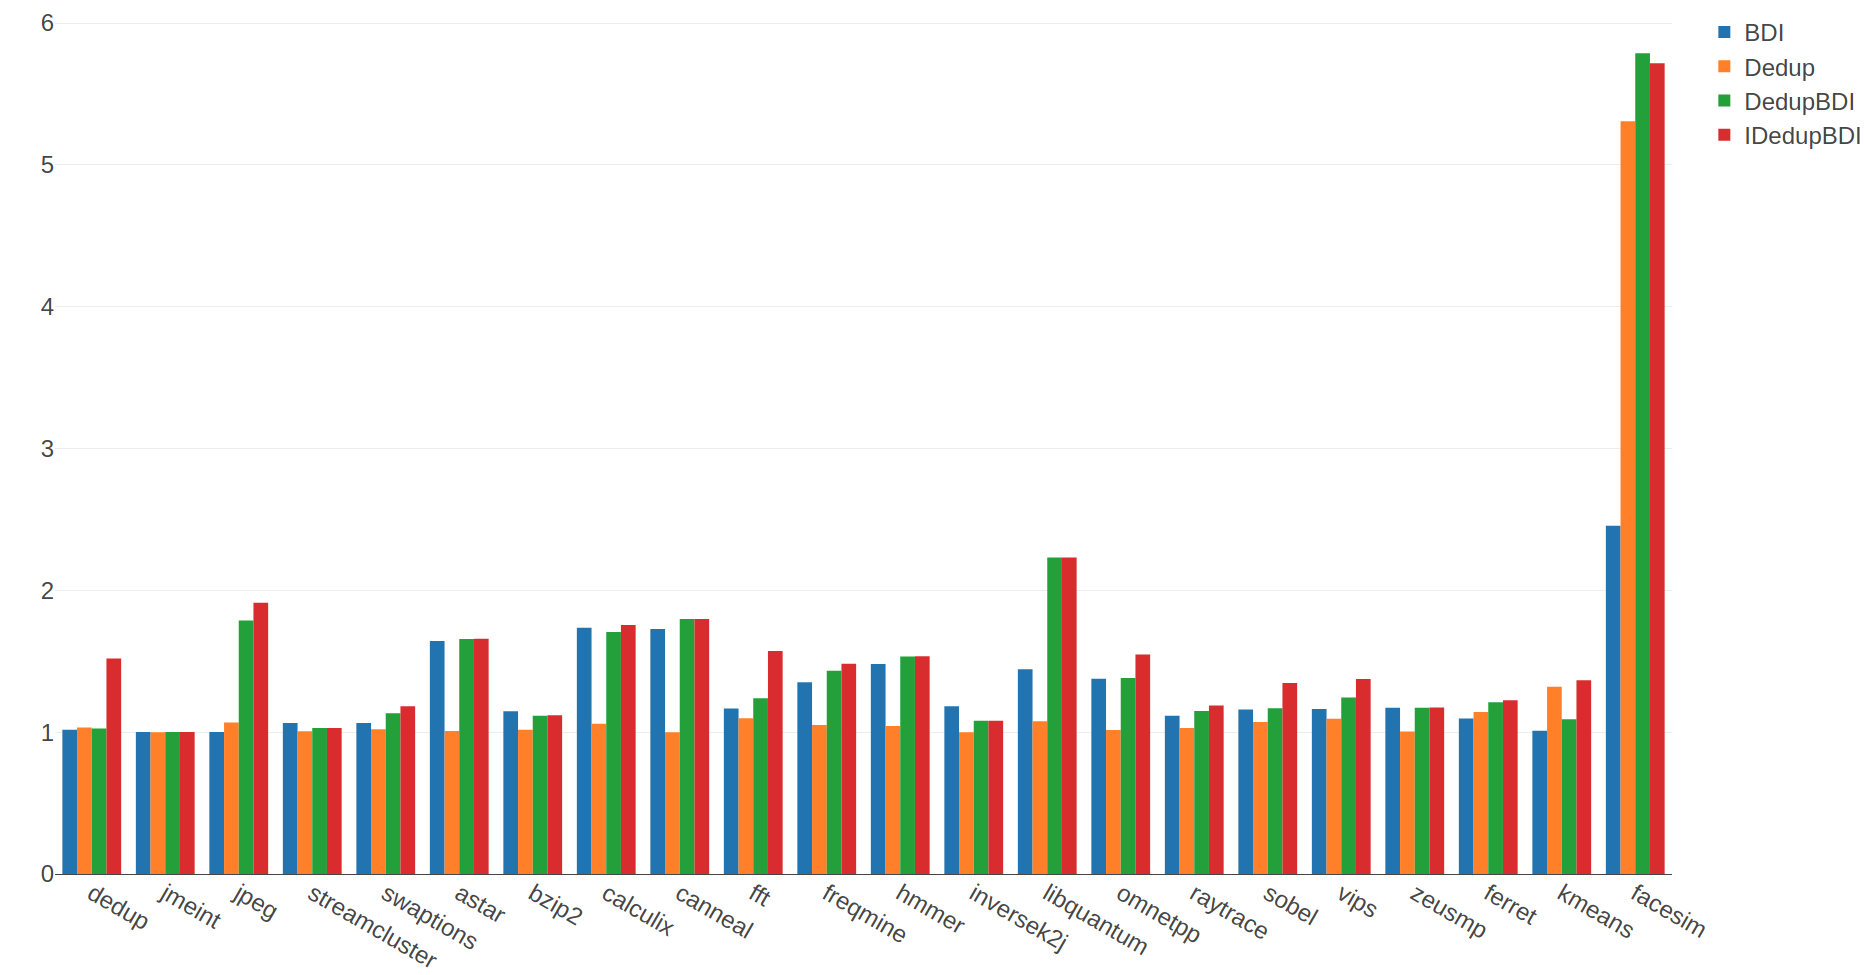
\includegraphics[width=\textwidth]{all-compratio1.png}
    \end{subfigure}
    \begin{subfigure}{\textwidth}
        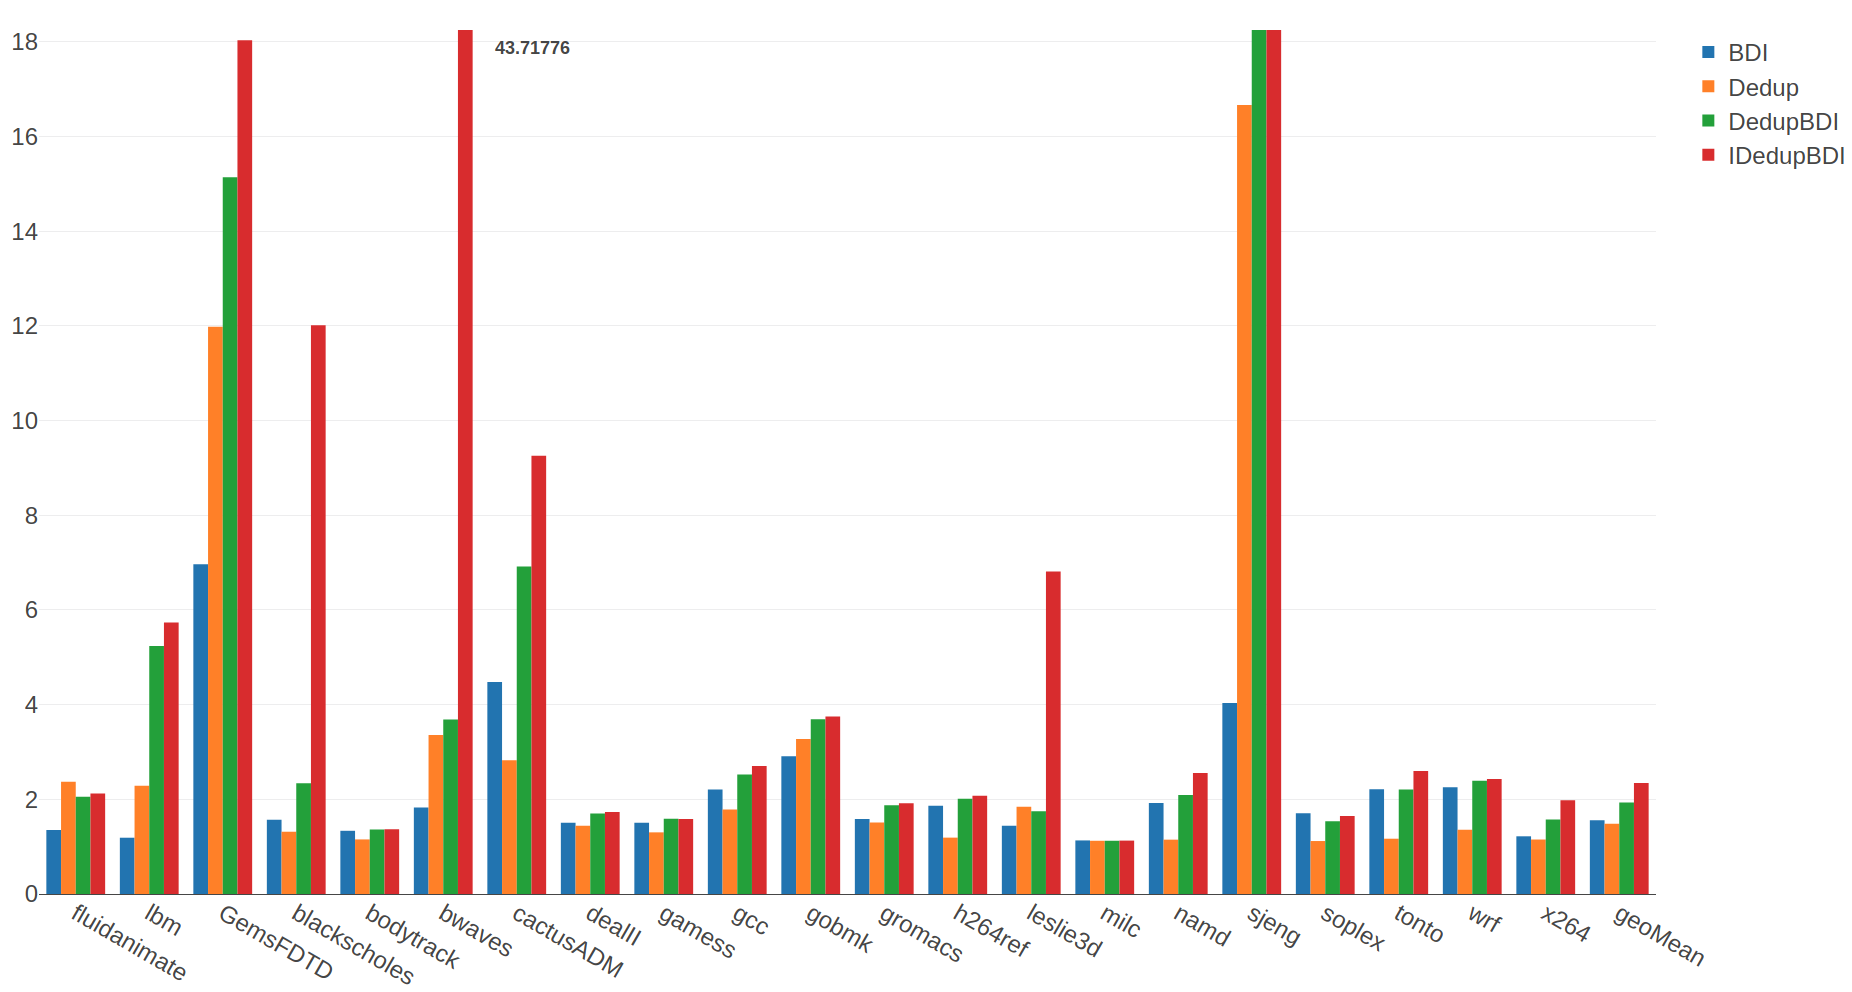
\includegraphics[width=\textwidth]{all-compratio2.png}
    \end{subfigure}
    \begin{subfigure}{\textwidth}
        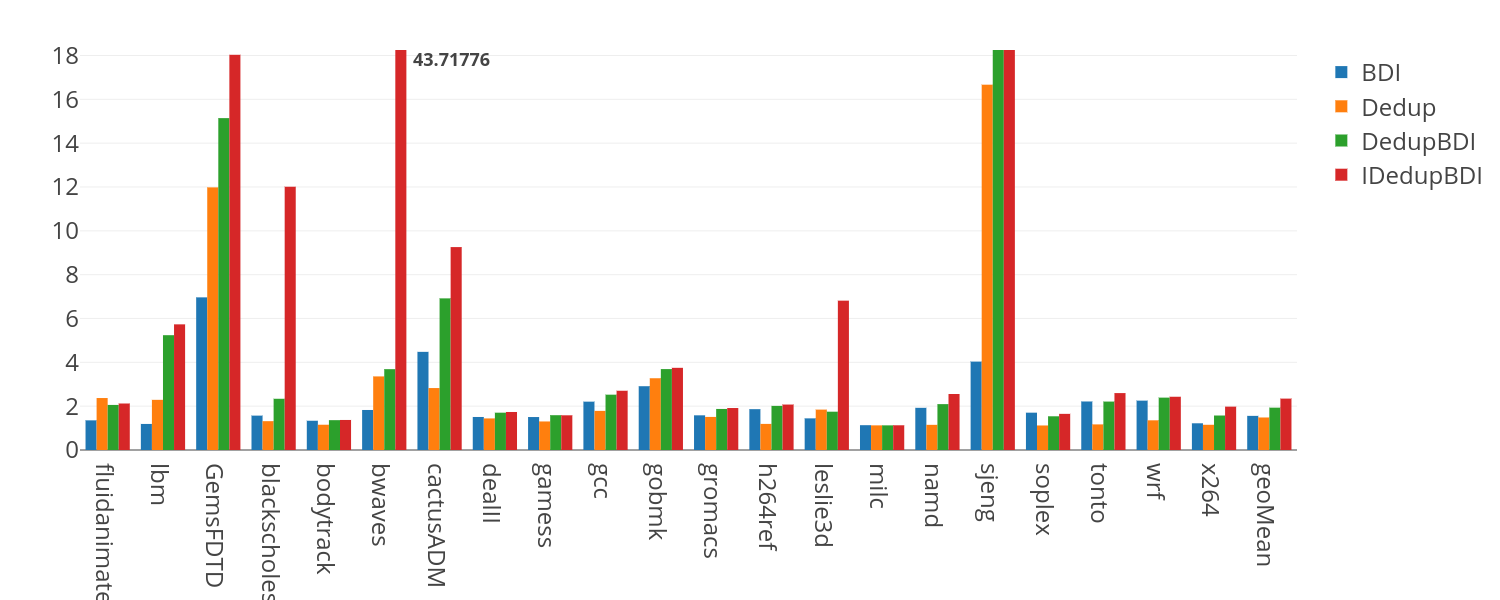
\includegraphics[width=\textwidth]{all-compratio3.png}
    \end{subfigure}
    \caption[All benchmarks: Compression]{Showing compression ratio for all benchmarks using all types of compressed 4MB caches with \#Tags = 4*\#Data Blocks. The third figure is the same as the second but zoomed out.}
    \label{fig:all_compratio}
\end{figure}
\begin{figure}
    \begin{subfigure}{\textwidth}
        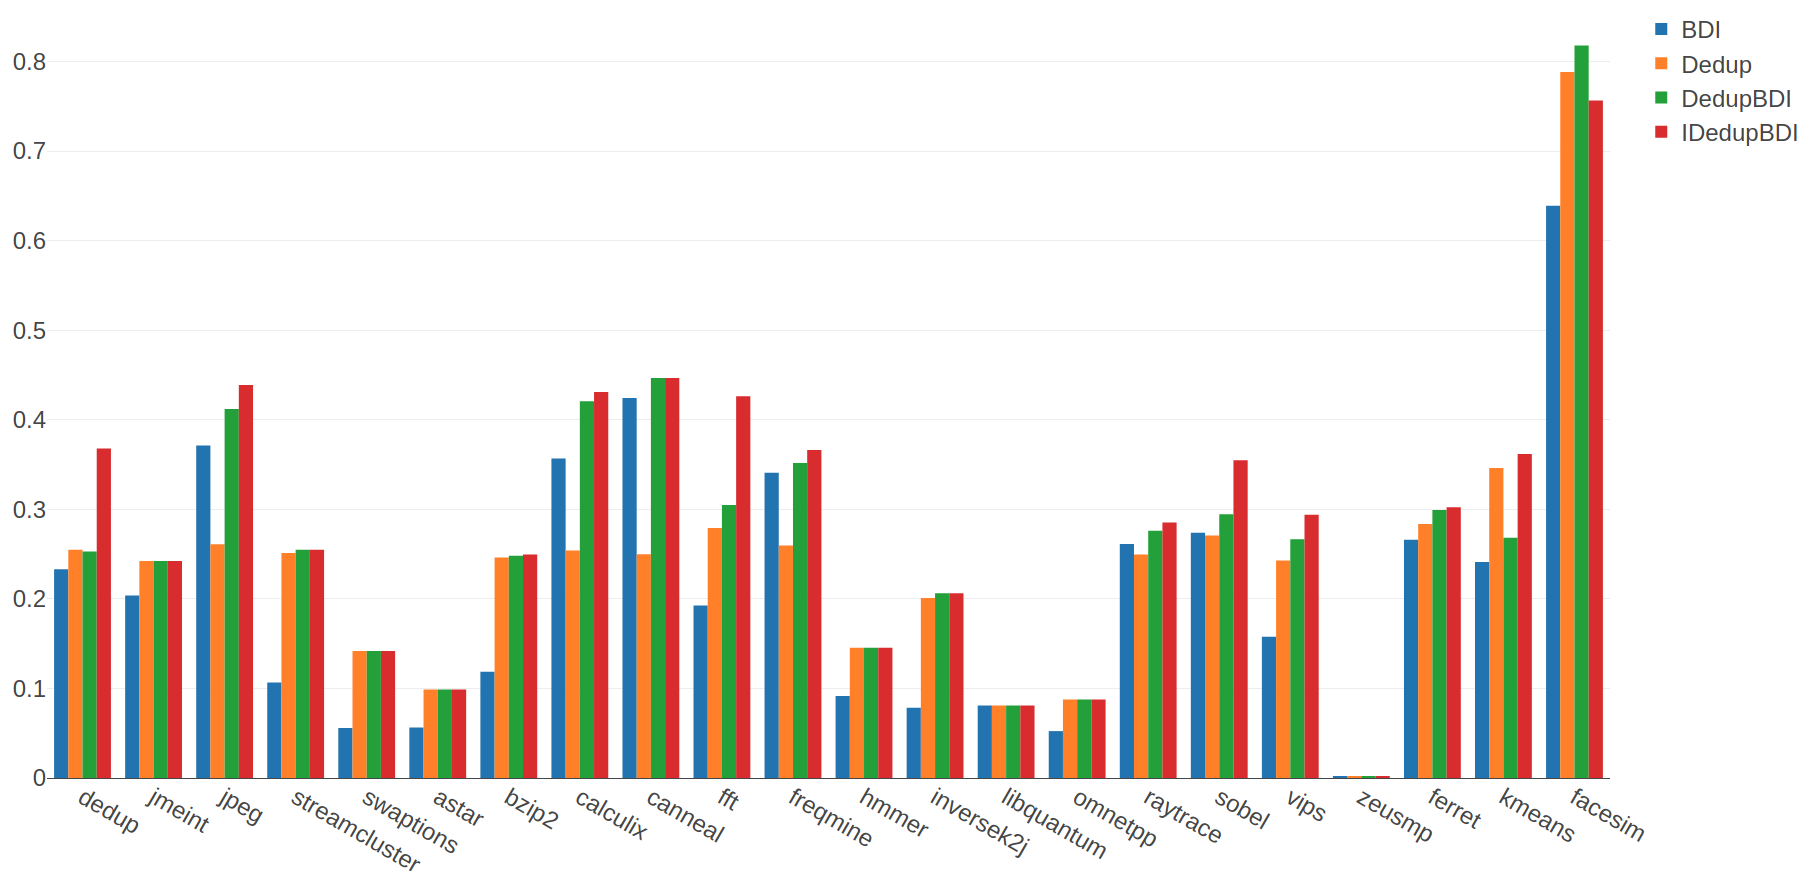
\includegraphics[width=\textwidth]{all-tagutil1.png}
    \end{subfigure}
    \begin{subfigure}{\textwidth}
        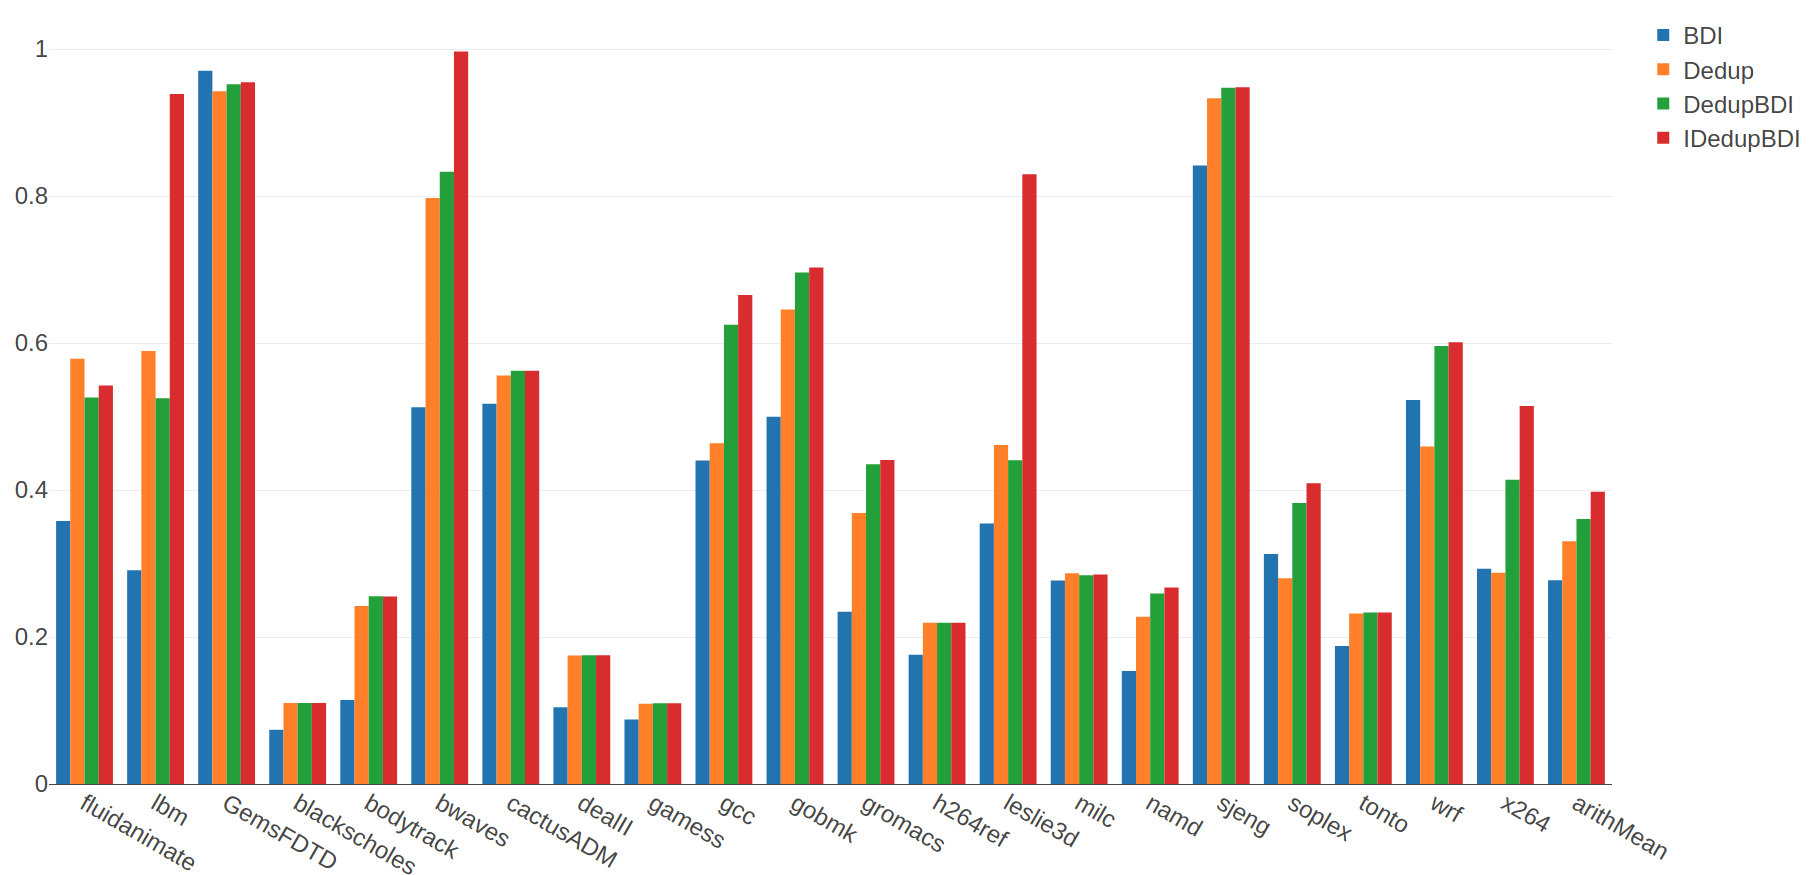
\includegraphics[width=\textwidth]{all-tagutil2.png}
    \end{subfigure}
    \caption[All benchmarks: Tag Utilization]{Showing tag utilization ratio for all benchmarks using all types of compressed 4MB caches with \#Tags = 4*\#Data Blocks.}
    \label{fig:all_tagutil}
\end{figure}
\begin{figure}
    \begin{subfigure}{\textwidth}
        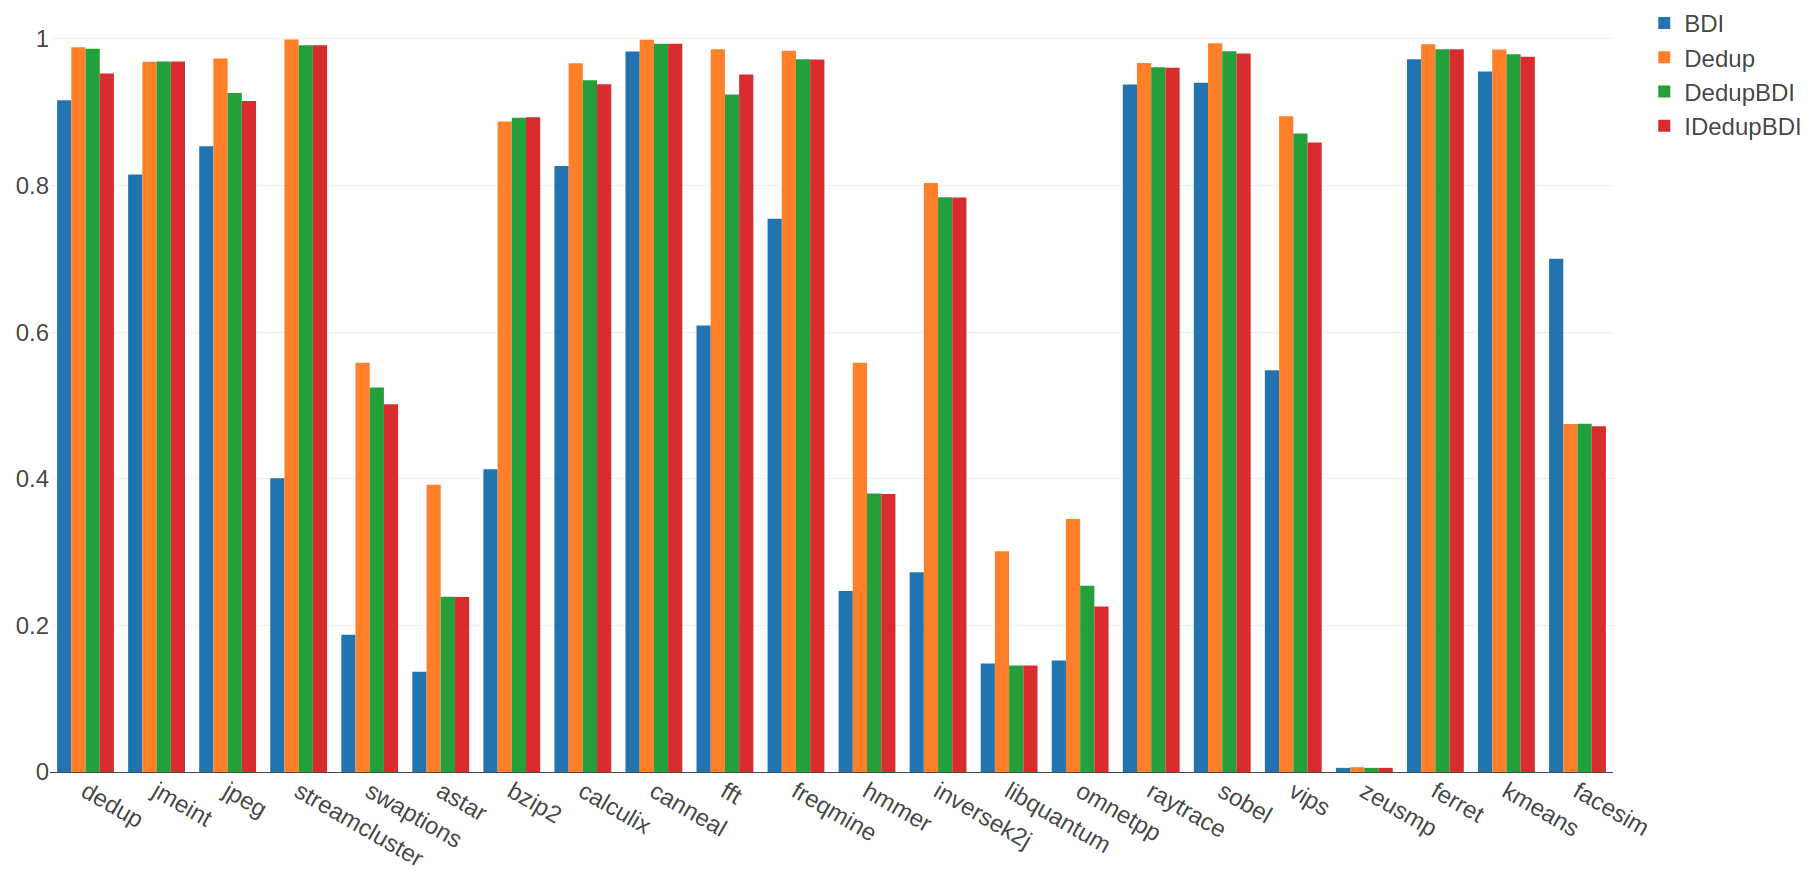
\includegraphics[width=\textwidth]{all-datautil1.png}
    \end{subfigure}
    \begin{subfigure}{\textwidth}
        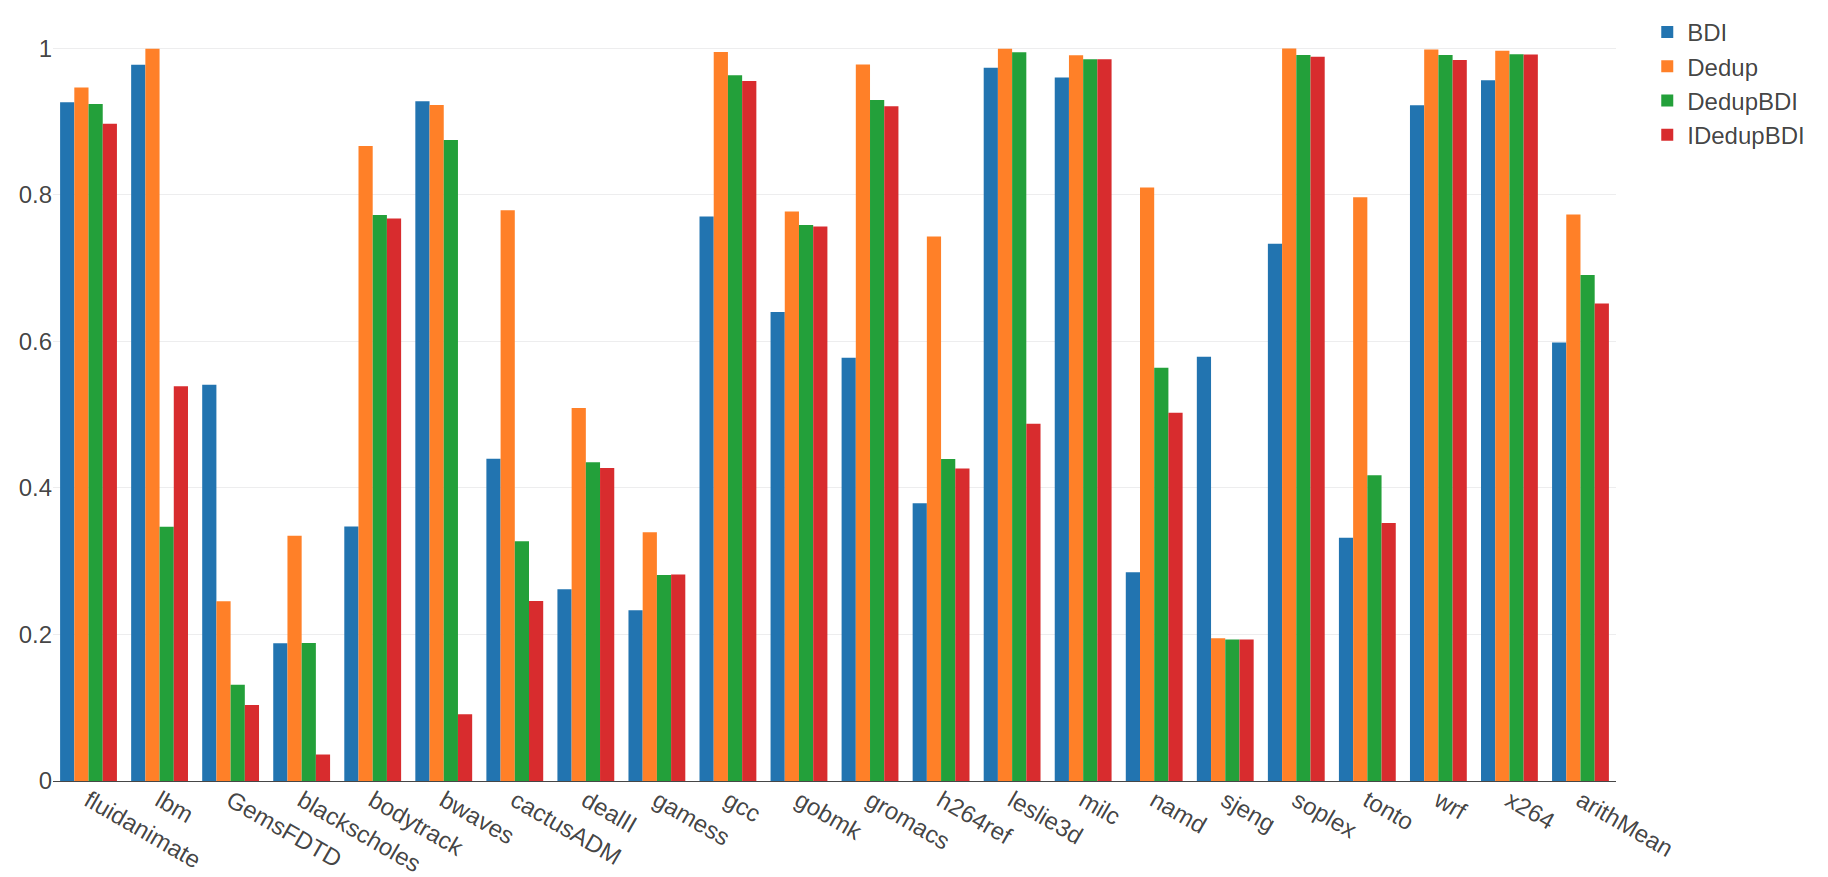
\includegraphics[width=\textwidth]{all-datautil2.png}
    \end{subfigure}
    \caption[All benchmarks: Data Utilization]{Showing data utilization ratio for all benchmarks using all types of compressed 4MB caches with \#Tags = 4*\#Data Blocks.}
    \label{fig:all_datautil}
\end{figure}
Figure~\ref{fig:all_compratio} shows the compression ratio for all the benchmarks when simulated with a compressed 4MB LLC with tags four times the data lines. The benchmarks are ordered by their compressibility. The first five benchmarks are hardly compressible by the BDI or the Dedup caches. The benchmarks from astar to zeusmp are only compressible by BDI. ferret and kmeans are only compressible by Dedup. The rest of the benchmarks are compressible using both techniques.\par
In all cases, it is shown that DedupBDI performs either better than BDI and Dedup, or at least similar to the dominant one. There are no cases in which DedupBDI compresses worse than BDI or Dedup. It can also be seen that the difference between DedupBDI and the ideal DedupBDI cache is minimal in most cases. Only in bwaves and fft benchmarks the upper bound perform a lot better than the real world implementation.\par
Benchmarks like bwaves, GemsFDTD, sjeng and facesim are compressible through both inter and intre-line compression but they are specifically very compressible and have a very high degree of deduplication. For example bwaves simulates a spherical blast wave and facesim simulates movements of a human face giving them a high degree of symmetry. Out of those four, only bwaves suffers from a very high hash miss ratio causing it to lose opportunity for a lot of deduplication, this shown in the huge difference between DedupBDI and IDedupBDI in Figure~\ref{fig:all_compratio}. Other benchmarks like fluidanimate, lbm, gcc, gobmk and tonto have enough symmetry and data patterns to be compressed through both BDI and Dedup. gobmk plays a Go game, fluidanimate does fluid dynamics for animation, tonto and lbm are scientific benchmarks for simulating quantum chemistry and incompressible fluids. All those applications have a degree of similarities to merit deduplication and compression. Figure~\ref{fig:BDIPotential} showed the patterns existing in some of those applications. Applications like astar, calculix, canneal, freqmine, hmmer, libquantum and omnetpp are all scientific applications that do not have obvious symmetry, but they show patterns compressible through BDI. These patterns are shown in Figure~\ref{fig:BDIPotential}.\par
However, the compression ratio does not tell the full story. If a cache contains 512 valid tags out of 1024, and 256 valid data lines out of 256 then it has a compression ratio of 2 but it is not being fully utilized. Normal conventional caches usually have near 100\% utilization unless the working data set is very small to entirely fit inside a cache. Figures~\ref{fig:all_tagutil} and~\ref{fig:all_datautil} shows the tag and data array utilization for all benchmarks. Most of the benchmarks can be divided into three categories:
\begin{itemize}
    \item \textbf{tag limited:} Those are benchmarks that have very high tag utilization, but lower than 100\% data utilization. facesim, GemsFDTD, bwaves and sjeng fall under this category. Those benchmarks are highly compressible and thus are bound by the size of the tag array. Evictions in such benchmarks are mainly caused by the tag array replacement policy.
    \item \textbf{data limited:} Those benchmarks reach near 100\% utilization of their data arrays before the tag array is full. This is because they have a lower degree of compressibility. For incompressible benchmarks like dedup and jmeint the tag array utilization sets around 25\% which is equivalent to the number of data lines, behaving exactly like an uncompressed cache of the same size and ignoring the extra tags. For other benchmarks like canneal, gromacs, and leslie3d the tag utilization is in mid ranges. Evictions in those benchmarks are prominently caused by the data array replacement policy.
    \item \textbf{Small Working Set:} Those are benchmark with small enough data to fit entirely in the L3 cache. Those show low tag and low data utilization ratios at the same time. Examples of benchmarks that fall under this category is zeusmp, blackscholes, omnetpp, and libquantum.
\end{itemize}
Results generated from other cache sizes (ranging from 0.5MB to 8MB) are very similar, we have chosen the 4MB-4 as a representative.\par
It is necessary to mention that our upper bound implementation only idealizes certain aspects as discussed in Section~\ref{sec:Upper Bound} but not all of them. For example, victimizing and evicting data lines is still done randomly. This causes the IDedupBDI implementation to sometimes perform worse than DedupBDI, like in the case of facesim in Figure~\ref{fig:all_compratio}.

\section{Performance}
\label{sec:Performance}
\begin{table}[]
    \centering
    \resizebox{\textwidth}{!}{%
    \begin{tabular}{|l|l|l|l|l|l|l|l|}
    \hline
    \multicolumn{1}{|c|}{Benchmark} & \multicolumn{1}{c|}{Cache Sensitive}                       & \textbf{Benchmark} & \textbf{Cache Sensitive}                                     & \textbf{Benchmark} & \textbf{Cache Sensitive}                                     & \textbf{Benchmark} & \textbf{Cache Sensitive}                                     \\ \hline
    fft                             & \begin{tabular}[c]{@{}l@{}}Big Sizes\\ (Semi)\end{tabular} & ferret             & \begin{tabular}[c]{@{}l@{}}All\\ (Semi)\end{tabular}         & zeusmp             & -                                                         & sphinx3            & Big Sizes                                                    \\ \hline
    inversek2j                      & -                                                       & fluidanimate       & -                                                         & gromacs            & \begin{tabular}[c]{@{}l@{}}Small Sizes\\ (Semi)\end{tabular} & wrf                & All                                                          \\ \hline
    jmeint                          & -                                                       & freqmine           & -                                                         & cactusADM          & \begin{tabular}[c]{@{}l@{}}All\\ (Semi)\end{tabular}         & bzip2              & All                                                          \\ \hline
    jpeg                            & -                                                       & raytrace           & -                                                         & leslie3d           & \begin{tabular}[c]{@{}l@{}}Big Sizes\\ (Semi)\end{tabular}   & gcc                & All                                                          \\ \hline
    kmeans                          & -                                                       & streamcluster      & -                                                         & namd               & -                                                         & gobmk              & \begin{tabular}[c]{@{}l@{}}Small Sizes\\ (Semi)\end{tabular} \\ \hline
    sobel                           & -                                                       & swaptions          & -                                                         & dealII             & Small Sizes                                                  & hmmer              & \begin{tabular}[c]{@{}l@{}}Small Sizes\\ (Semi)\end{tabular} \\ \hline
    blackscholes                    & -                                                       & vips               & \begin{tabular}[c]{@{}l@{}}Small Sizes\\ (Semi)\end{tabular} & soplex             & \begin{tabular}[c]{@{}l@{}}All\\ (Semi)\end{tabular}         & sjeng              & -                                                         \\ \hline
    bodytrack                       & -                                                       & x264               & -                                                         & calculix           & Small Sizes                                                  & libquantum         & Mid Sizes                                                    \\ \hline
    canneal                         & \begin{tabular}[c]{@{}l@{}}All\\ (Semi)\end{tabular}       & bwaves             & -                                                         & GemsFDTD           & -                                                         & h264ref            & \begin{tabular}[c]{@{}l@{}}All\\ (Semi)\end{tabular}         \\ \hline
    dedup                           & -                                                       & gamess             & \begin{tabular}[c]{@{}l@{}}Small Sizes\\ (Semi)\end{tabular} & tonto              & \begin{tabular}[c]{@{}l@{}}Small Sizes\\ (Semi)\end{tabular} & omnetpp            & Small Sizes                                                  \\ \hline
    facesim                         & -                                                       & milc               & -                                                         & lbm                & -                                                         & astar              & All                                                          \\ \hline
    \end{tabular}%
    }
    \caption{All benchmarks and their cache behavior}
    \label{tab:cachesense}
\end{table}
\begin{figure}
    \begin{subfigure}{\textwidth}
        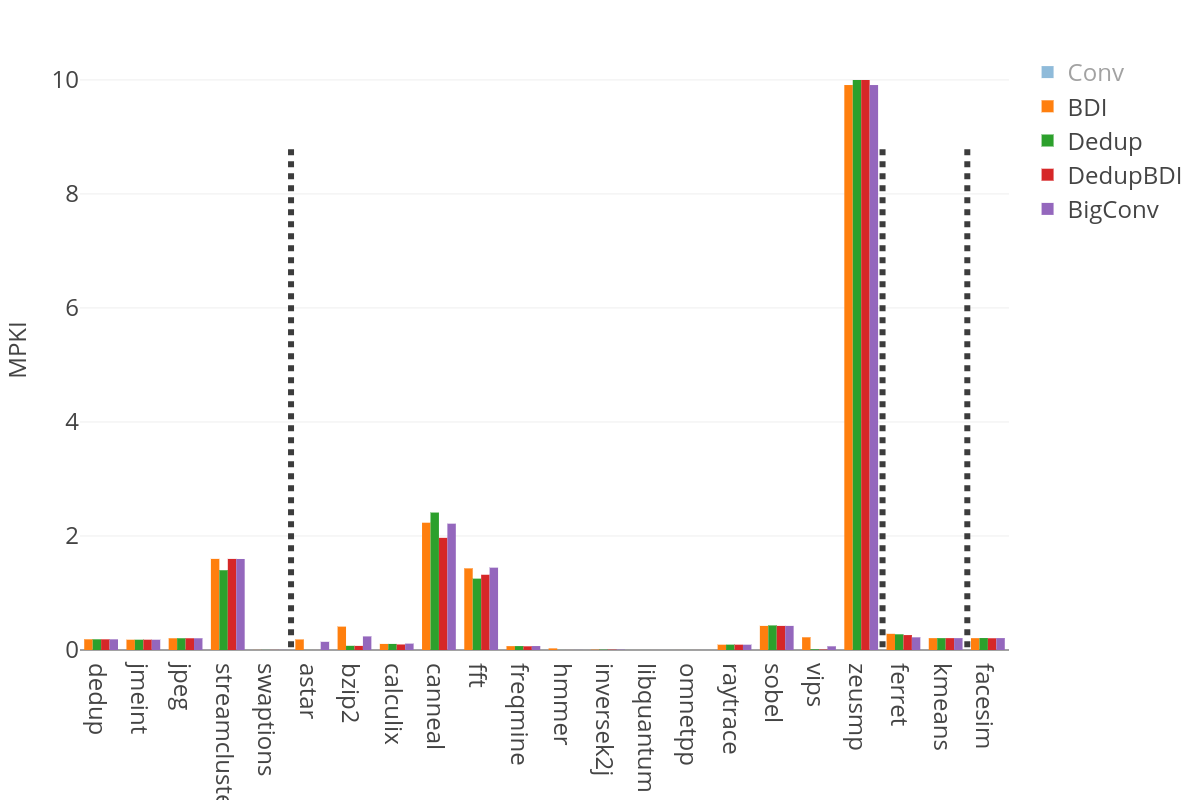
\includegraphics[width=\textwidth]{all4-mpki1.png}
    \end{subfigure}
    \begin{subfigure}{\textwidth}
        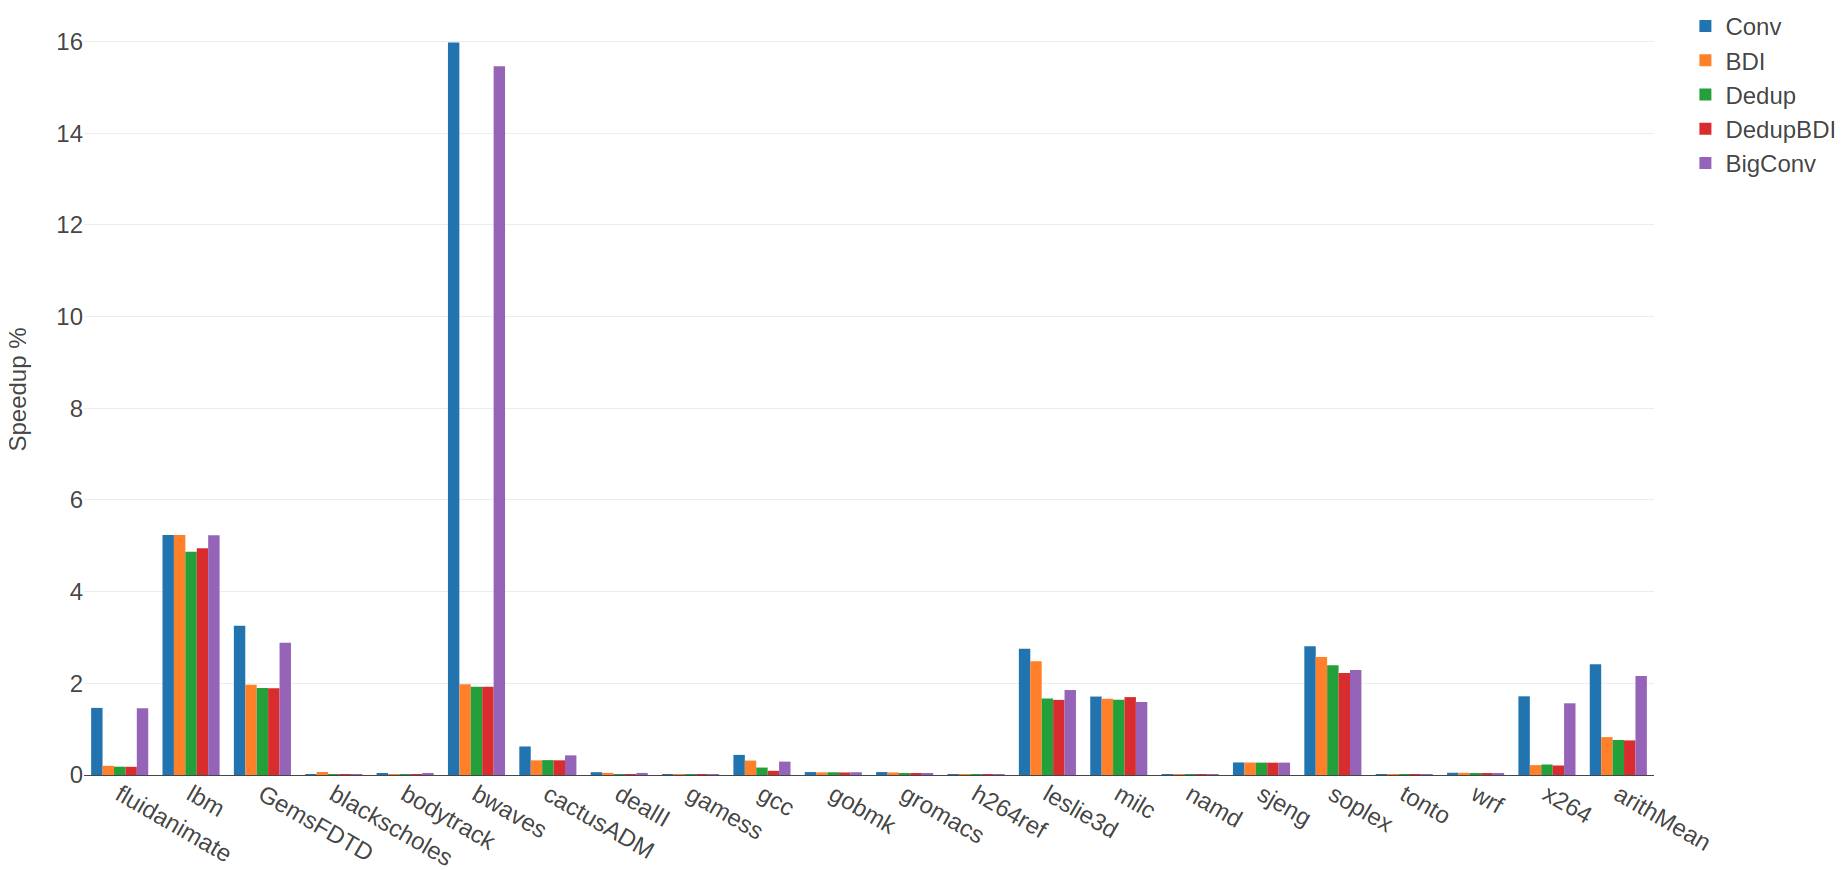
\includegraphics[width=\textwidth]{all4-mpki2.png}
    \end{subfigure}
    \caption[All benchmarks: 4MB MPKI]{Showing MPKI for all types of compressed 4MB caches with \#Tags = 4*\#Data Blocks against conventional same size caches and conventional cache with double the size.}
    \label{fig:all_mpki}
\end{figure}
\begin{figure}
    \begin{subfigure}{\textwidth}
        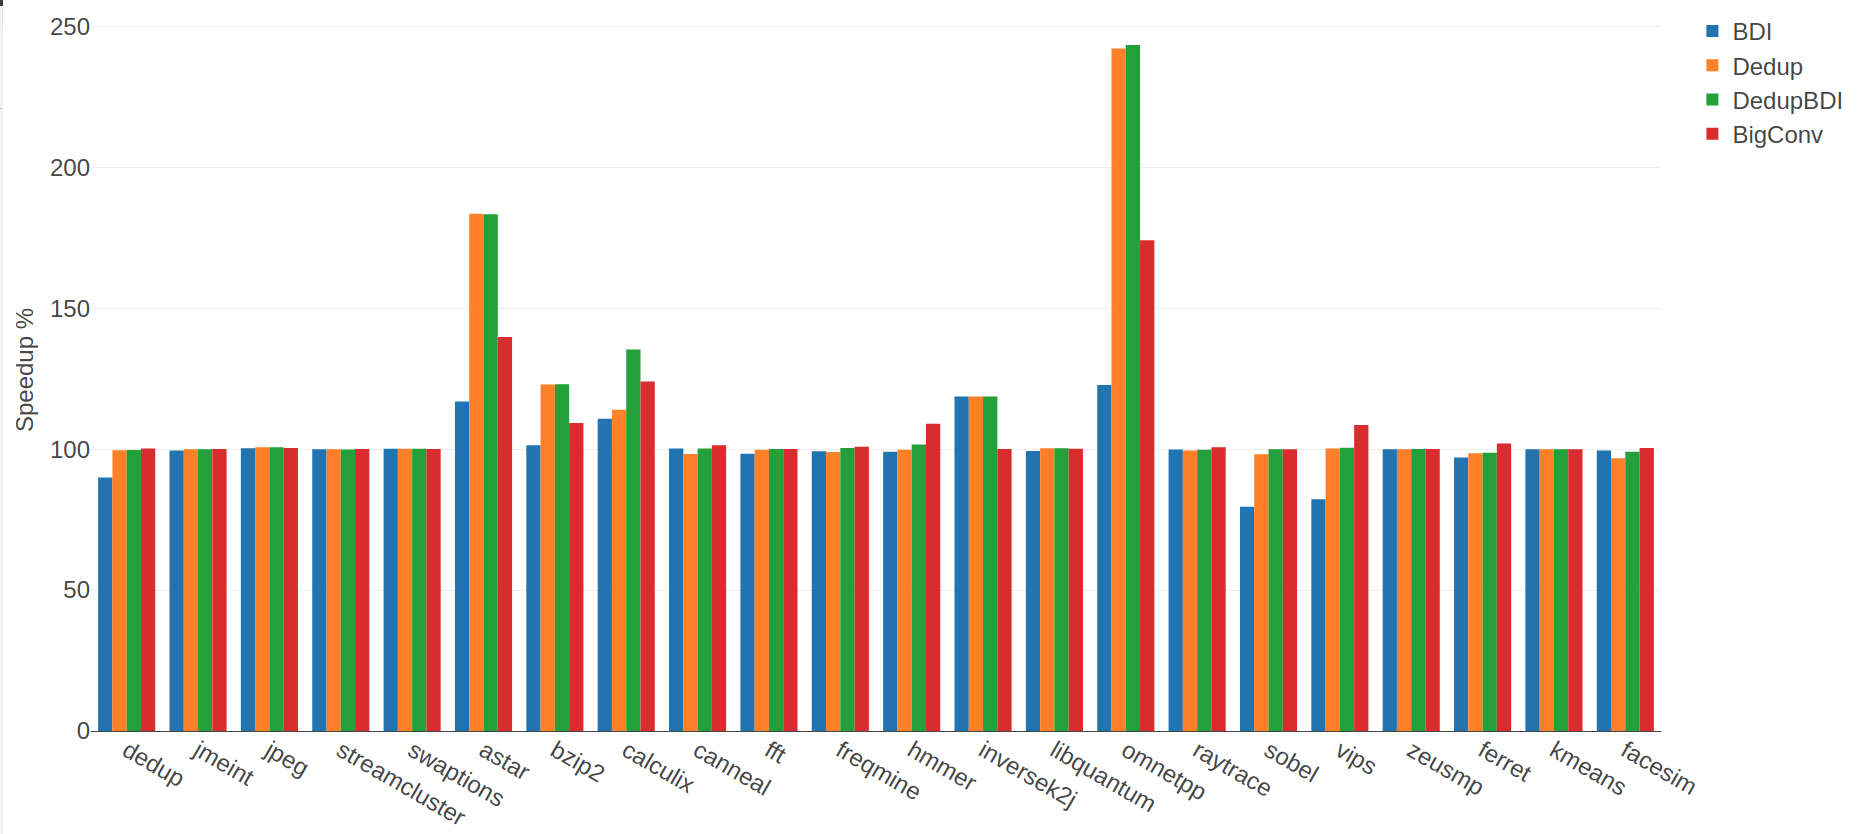
\includegraphics[width=\textwidth]{all5-speedup1.png}
    \end{subfigure}
    \begin{subfigure}{\textwidth}
        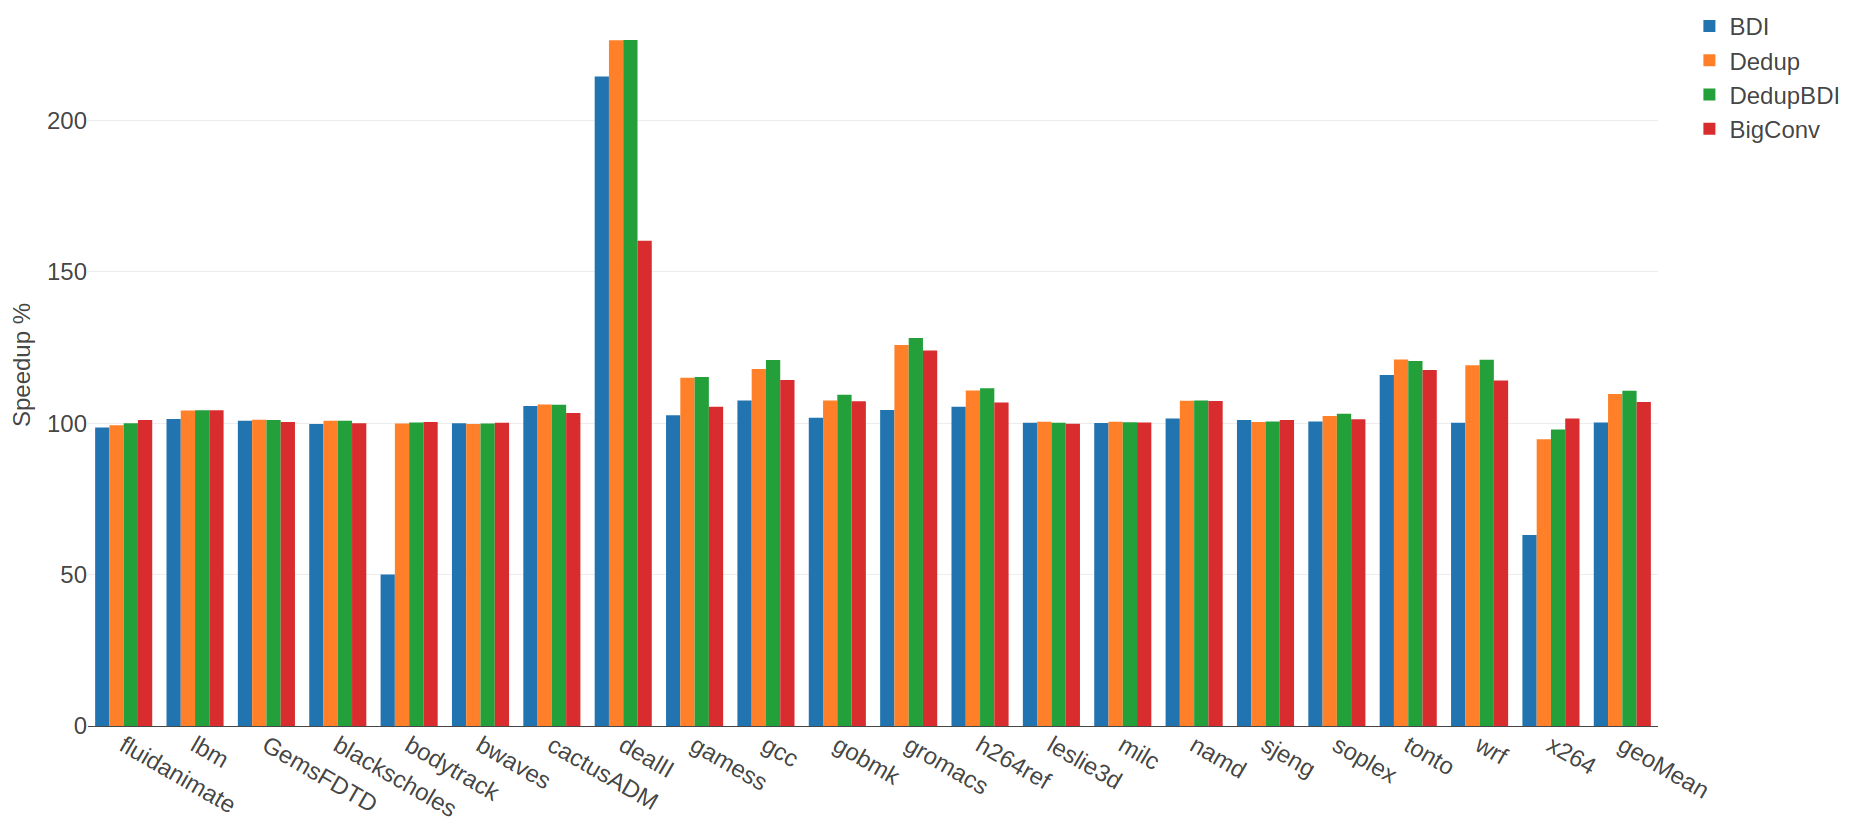
\includegraphics[width=\textwidth]{all5-speedup2.png}
    \end{subfigure}
    \caption[All benchmarks: 0.5MB Speedup]{Showing Speedup for all types of compressed 0.5MB caches with \#Tags = 4*\#Data Blocks against conventional same size caches and conventional cache with double the size.}
    \label{fig:all_speedup1}
\end{figure}
\begin{figure}
    \begin{subfigure}{\textwidth}
        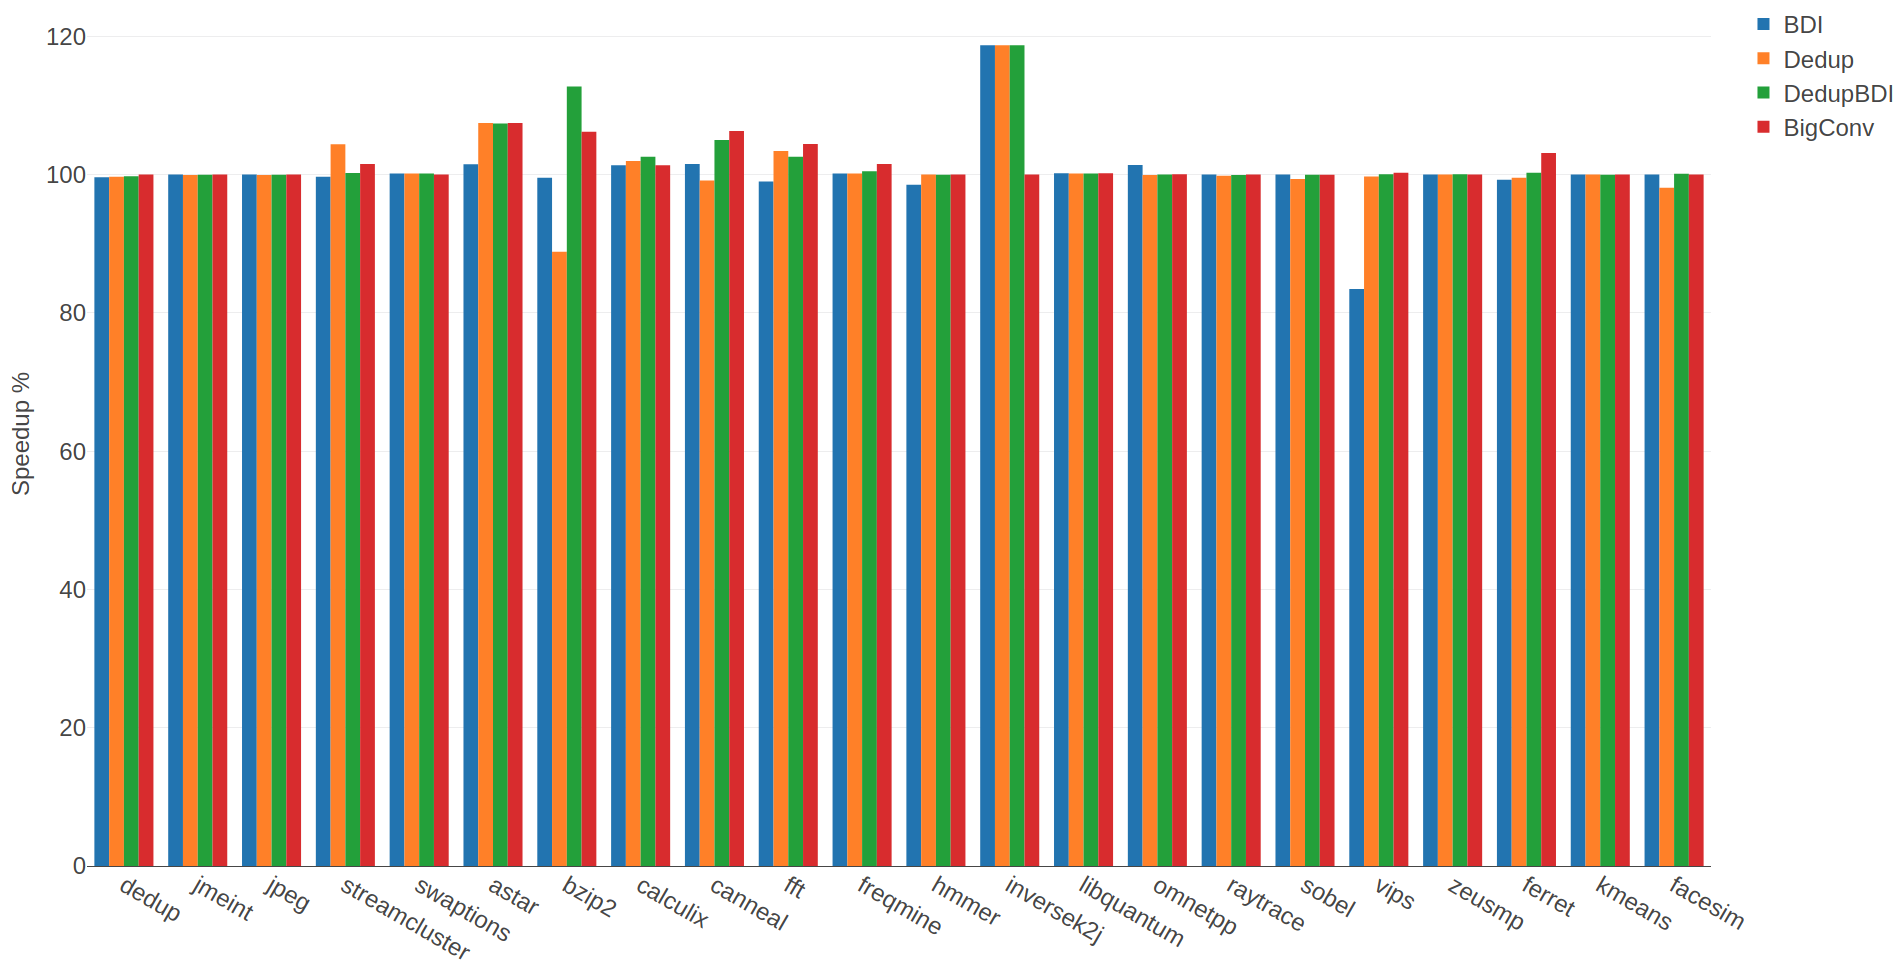
\includegraphics[width=\textwidth]{all4-speedup1.png}
    \end{subfigure}
    \begin{subfigure}{\textwidth}
        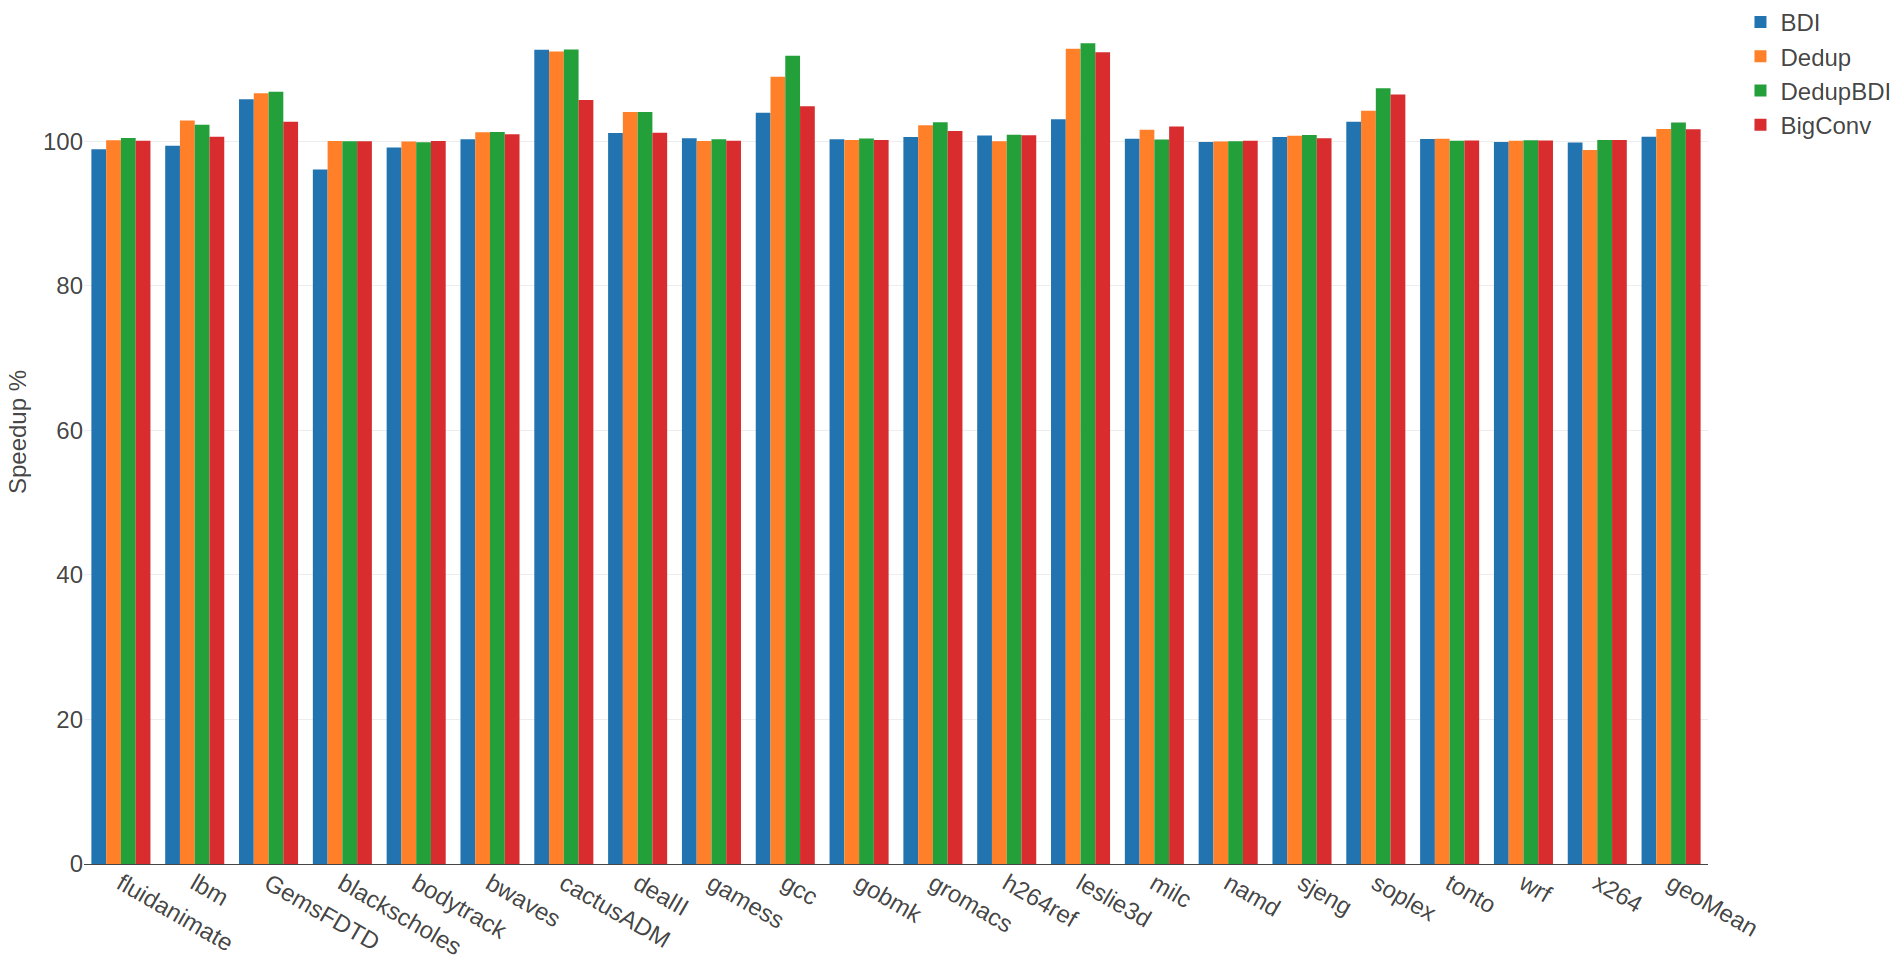
\includegraphics[width=\textwidth]{all4-speedup2.png}
    \end{subfigure}
    \caption[All benchmarks: 0.5MB Speedup]{Showing Speedup for all types of compressed 4MB caches with \#Tags = 4*\#Data Blocks against conventional same size caches and conventional cache with double the size.}
    \label{fig:all_speedup2}
\end{figure}
Figure~\ref{fig:all_mpki} shows the MPKI for all the benchmarks when simulated with conventional and compressed 4MB LLC caches with tags four times the data lines. Benchmarks are ordered similarly to~\ref{fig:all_compratio}. The figure shows that compressed caches reduce MPKI in LLC. DedupBDI is either the same as Dedup or BDI or is outperforming them. In general DedupBDI performs better than a conventional cache of twice the size.\par
However, the decrease of MPKI doesn't always necessitate speedup. The benchmark access patterns and cache sensitivity also play a role. Table~\ref{tab:cachesense} shows the behavior of all benchmarks over a range of cache sizes. Every benchmark is classified as cache sensitive, cache insensitive, or cache sensitive at a specific cache size range.
Figures~\ref{fig:all_speedup1} and~\ref{fig:all_speedup2} show the speedup for all the benchmarks when simulated with a compressed 0.5MB and 4MB LLC caches with tags four times the data lines, respectively. We have chosen those two sizes because some benchmarks are only cache sensitive with lower cache sizes while others are only cache sensitive at higher cache sizes.\par
For the cache insensitive benchmarks, the DedupBDI cache performs as fast as the conventional caches. It does not provide any more speedup. But it allows the data to be compressed, providing area and power savings. For the cache sensitive benchmarks, DedupBDI outperforms the conventional, Dedup, and DedupBDI caches altogether.

\section{Tag to Data Ratio}
\label{sec:tagratio}
\begin{figure}
    \begin{subfigure}{\textwidth}
        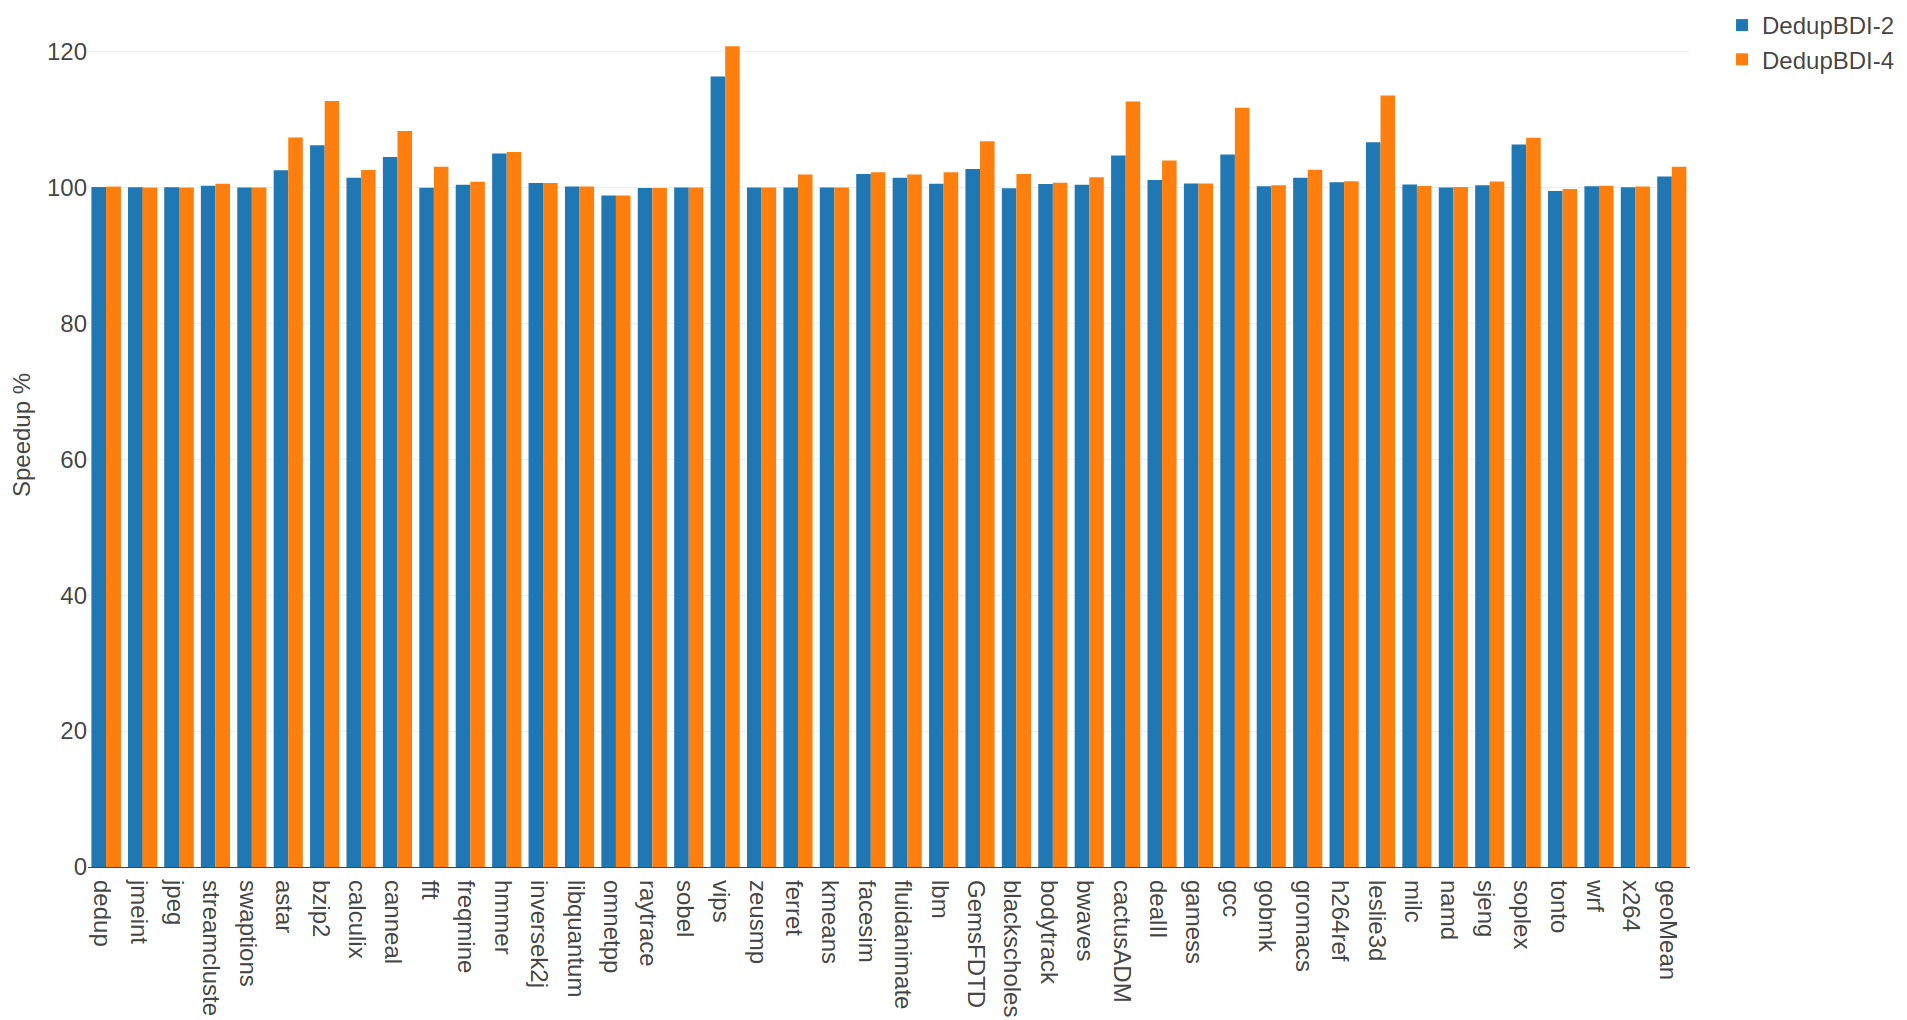
\includegraphics[width=\textwidth]{compare-speedup.png}
    \end{subfigure}
    \begin{subfigure}{\textwidth}
        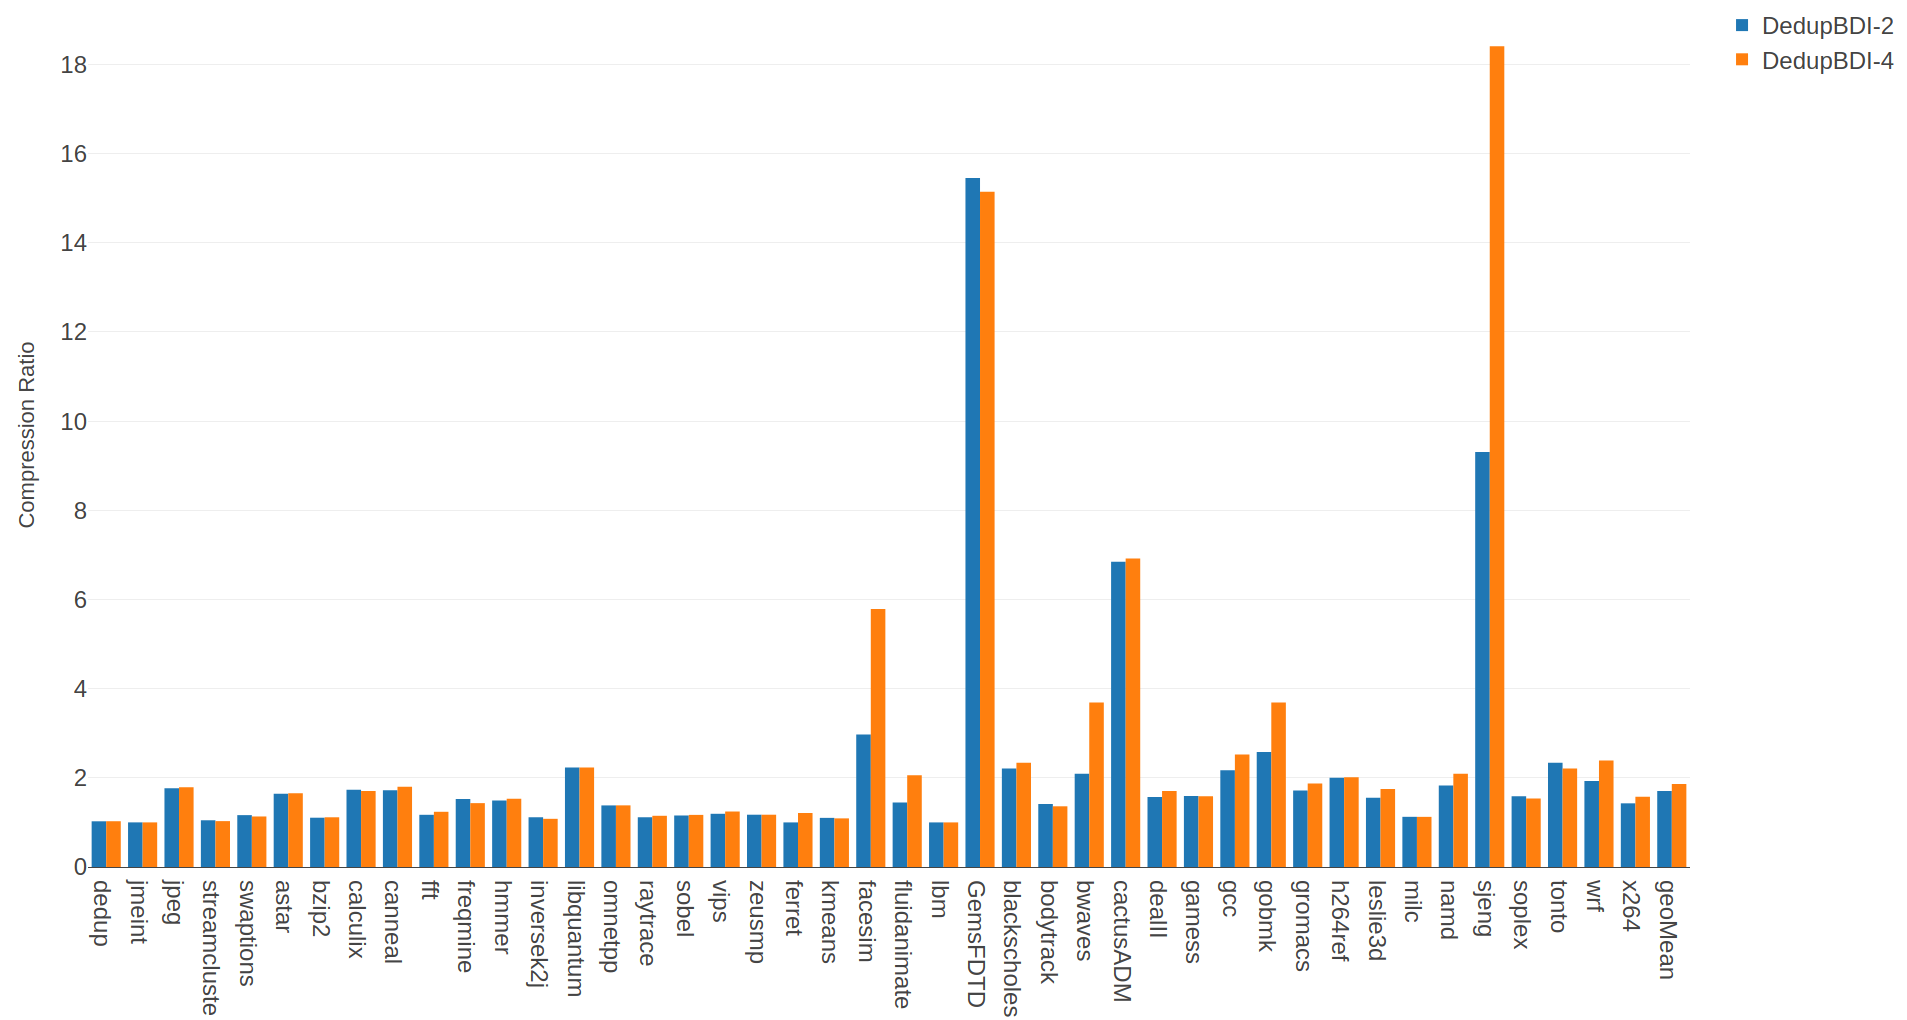
\includegraphics[width=\textwidth]{compare-compression.png}
    \end{subfigure}
    \caption[All benchmarks: Tag Ratio]{Showing performance and compression ratio for all benchmarks using DedupBDI 4MB caches with \#Tags = 4*\#Data Blocks and twice the data.}
    \label{fig:all_compare}
\end{figure}
Figure~\ref{fig:all_compare} shows the difference between two 4MB DedupBDI caches, one with tags twice the data entries (4MB-2) and the other with tags four times the data entries(4MB-4). Using the tags as four times the data entries requires compression to be highly effective. Otherwise the cache will run out of data space quickly and throttle the performance. As Figure~\ref{fig:all_compare} shows, the smaller 4MB-4 cache achieves better performance than the 4MB-2 and has better compression ratio. We've chosen caches with four times the tags to be our default compressed cache size.


\section{Overhead Analysis}
\label{sec:Overhead}
\begin{table}[]
    \centering
    \begin{tabular}{lllll}
               & Conv   & BDI    & Dedup  & DedupBDI \\ \hline
    Tags       &        &        &        &          \\
    \# Entries & 8192   & 32768   & 32768   & 32768     \\
    Entry Size & 49b    & 47b    & 47b    & 47b      \\
    Overhead   & 6b     & 15b    & 35b    & 42b      \\
    Total Size & 55KB   & 248KB   & 328KB   & 356KB     \\ \hline
    Data       &        &        &        &          \\
    \# Entries & 8192   & 8192   & 8192   & 8192     \\
    Entry Size & 64B    & 64B    & 64B    & 64B      \\
    Overhead   &        &        & 11b    & 11B      \\
    FreeList   &        &        & 2.75KB & 896B     \\
    Total Size & 0.5MB  & 0.5MB  & 525.75KB & 600.875KB   \\ \hline
    Hash       &        &        &        &          \\
    \# Entries &        &        & 64     & 64       \\
    Entry Size &        &        & 10b    & 10b      \\
    Overhead   &        &        & 11b    & 14b      \\
    Total Size &        &        & 168B   & 192B     \\ \hline
    Total Bank Size & 567KB & 760KB & 853.91KB & 980.875KB  
    \end{tabular}
    \caption{4MB cache size and overhead in all configurations.}
    \label{tab:overhead}
\end{table}
Table~\ref{tab:overhead} shows the overheads in one bank in the four cache designs we studied, assuming an 8 banked cache, with an associativity of 16, cache size of 4MB, and LRU replacement policy. The overhead in all caches comes from four different sources:
\begin{itemize}
    \item \textbf{Tag Overhead:}
    \begin{itemize}
        \item \textbf{conventional:} In conventional caches, assuming LRU replacement policy, the tag overhead per entry consists of one bit for Valid, one for Dirty, and log2(associativity) bits for the LRU replacement. 
        \item \textbf{BDI:} In BDI there is an extra overhead of 4 bits for compression encoding and log2(associativity*\#SegmentsPerLine) bits for segment pointers. Along with the normal overhead from a conventional cache. Note that in BDI the data array has half or one quarter of the associativity of the tag array.
        \item \textbf{Dedup:} On top of the conventional cache overhead, Dedup adds two pointers per tag entry for the next/previous tag to build a linked list, each one of those is log2(\#Tags/associativity) bits. It also adds pointers to the data line associated with it. Since Dedup data arrays are direct mapped the data pointer size is log2(\#Data).
        \item \textbf{DedupBDI:} DedupBDI adds the same overhead as the BDI cache. It also adds the same linked list pointers from the Dedup cache, but its data pointer size is different from the Dedup cache. Because the data array in DedupBDI maintains its associativity, the data pointer size is log2(\#Data/associativity).
    \end{itemize}
    \item \textbf{Data Overhead:}
    \begin{itemize}
        \item \textbf{conventional:} A conventional cache has no overheads in its data array.
        \item \textbf{BDI:} Similar to a conventional cache, A BDI cache does not have any metadata in its data array and thus does not have any overhead.
        \item \textbf{Dedup:} The data lines in a Dedup cache requires a pointer to the tag, which is enough to point to the tag set so it has a size of log2(\#Tags/associativity). It also requires each data line to have a deduplication counter, which we described in~\ref{ch:BackgroundMotiv} to be 2 bits.
        \item \textbf{DedupBDI:} The DedupBDI data array has the same overhead as its Dedup counterpart. Except the overhead is per segment instead of being per line. that means for each data line we have 8 Dedup data overheads.
    \end{itemize}
    \item \textbf{Extra Data Overhead:}
    \begin{itemize}
        \item \textbf{Dedup:} The Dedup cache maintains a free list of its free data lines. The free list is essentially a FIFO with the same number of entries as data lines, and with a width that is enough to hold a pointer to the corresponding data line (i.e. log2(\#Data)).
        \item \textbf{DedupBDI:} The DedupBDI cache maintains 8 different free lists. Each of them is a FIFO with the same number of sets as data sets (i.e. Data lines/associativity), with a width that is enough to hold a pointer to the set (i.e. log2(\#Data/associativity)).
    \end{itemize}
    \item \textbf{Hash Array:} The Dedup and DedupBDI have the same hash array design. The hash array saves part of the hash as a tag while the other part is used as an index. The hash array then has the size of \#Hash*(HashSize-log2(\#Hash/associativity)). The Dedup and DedupBDI hash arrays then have some extra overhead:
    \begin{itemize}
        \item \textbf{Dedup:} each hash entry has a data pointer of size log2(\#Data)
        \item \textbf{DedupBDI:} each hash entry has a data pointer of size log2(\#Data/associativity) and segment pointer of size log2(associativity*\#SegmentsPerLine) bits.
    \end{itemize}
\end{itemize}
It is obvious that DedupBDI has the highest amount of overhead. But it also gains the most savings and speedups.

\section{Area and Power}
\label{sec:areapower}
\begin{table}[]
    \centering
    \resizebox{\textwidth}{!}{%
    \begin{tabular}{llllll}
    \multicolumn{2}{c}{Cache}                                                 & \multicolumn{1}{c}{\begin{tabular}[c]{@{}c@{}}Access Latency\\ (ns)\end{tabular}} & \multicolumn{1}{c}{\begin{tabular}[c]{@{}c@{}}Dynamic Read\\ Energy (nJ)\end{tabular}} & \multicolumn{1}{c}{\begin{tabular}[c]{@{}c@{}}Leakage Power\\ (mW)\end{tabular}} & \multicolumn{1}{c}{Area (mm2)} \\ \hline
    \multicolumn{1}{l|}{\multirow{5}{*}{CONV}}     & \multicolumn{1}{l|}{0.5} & 1.04                                                                         & 0.28                                                                              & 353.33                                                                        & 12.20                     \\
    \multicolumn{1}{l|}{}                          & \multicolumn{1}{l|}{1}   & 1.12                                                                          & 0.3                                                                              & 530.38                                                                        & 13.07                      \\
    \multicolumn{1}{l|}{}                          & \multicolumn{1}{l|}{2}   & 1.29                                                                          & 0.33                                                                              & 884.79                                                                        & 14.77                      \\
    \multicolumn{1}{l|}{}                          & \multicolumn{1}{l|}{4}   & 1.46                                                                           & 0.4                                                                               & 1579.64                                                                        & 18.13                      \\
    \multicolumn{1}{l|}{}                          & \multicolumn{1}{l|}{8}   & 1.92                                                                          & 0.53                                                                                & 2978.40                                                                        & 24.88                      \\ \cline{1-2}
    \multicolumn{1}{l|}{\multirow{5}{*}{BDI}}      & \multicolumn{1}{l|}{0.5} & 1.13                                                                          & 0.29                                                                              & 418.39                                                                         & 12.54                      \\
    \multicolumn{1}{l|}{}                          & \multicolumn{1}{l|}{1}   & 1.31                                                                          & 0.31                                                                               & 660.59                                                                         & 13.73                      \\
    \multicolumn{1}{l|}{}                          & \multicolumn{1}{l|}{2}   & 1.4                                                                          & 0.35                                                                               & 1140.98                                                                        & 16.03                      \\
    \multicolumn{1}{l|}{}                          & \multicolumn{1}{l|}{4}   & 1.78                                                                          & 0.44                                                                               & 2096.47                                                                        & 20.58                      \\
    \multicolumn{1}{l|}{}                          & \multicolumn{1}{l|}{8}   & 2.23                                                                          & 0.602                                                                               & 3939.53                                                                         & 29.58                      \\ \cline{1-2}
    \multicolumn{1}{l|}{\multirow{5}{*}{DEDUP}}    & \multicolumn{1}{l|}{0.5} & 1.16                                                                          & 0.29                                                                              & 442.7                                                                         & 12.65                      \\
    \multicolumn{1}{l|}{}                          & \multicolumn{1}{l|}{1}   & 1.40                                                                          & 0.31                                                                               & 719.35                                                                         & 14                      \\
    \multicolumn{1}{l|}{}                          & \multicolumn{1}{l|}{2}   & 1.49                                                                          & 0.36                                                                               & 1273.9                                                                        & 16.65                      \\
    \multicolumn{1}{l|}{}                          & \multicolumn{1}{l|}{4}   & 1.83                                                                          & 0.46                                                                               & 2355.5                                                                         & 21.96                      \\
    \multicolumn{1}{l|}{}                          & \multicolumn{1}{l|}{8}   & 2.21                                                                          & 0.59                                                                               & 4583.88                                                                         & 32.95                      \\ \cline{1-2}
    \multicolumn{1}{c|}{\multirow{5}{*}{DEDUPBDI}} & \multicolumn{1}{l|}{0.5} & 1.18                                                                          & 0.29                                                                               & 471.35                                                                         & 12.79                      \\
    \multicolumn{1}{c|}{}                          & \multicolumn{1}{l|}{1}   & 1.44                                                                          & 0.32                                                                               & 778.99                                                                         & 14.28                      \\
    \multicolumn{1}{c|}{}                          & \multicolumn{1}{l|}{2}   & 1.53                                                                          & 0.37                                                                               & 1403.04                                                                        & 17.26                      \\
    \multicolumn{1}{c|}{}                          & \multicolumn{1}{l|}{4}   & 1.89                                                                          & 0.49                                                                               & 2628.79                                                                         & 23.26                      \\
    \multicolumn{1}{c|}{}                          & \multicolumn{1}{l|}{8}   & 2.33                                                                          & 0.63                                                                                & 5160.35                                                                         & 35.73                      \\ \cline{1-2}
    \end{tabular}%
    }
    \caption{Area, Power, Energy, and Access Latency for all cache sizes and configurations.}
    \label{tab:areapower}
\end{table}
We used cacti6\cite{cacti} to get power and area estimations for all the cache types and sizes we simulated. We used CACTI to only model the cache arrays, but not the compression/decompression or hashing hardware. We used the target technology as 32nm. The results are shown in~\ref{tab:areapower}. The results in the table are consistent with what we've discussed so far. DedupBDI caches have higher access latencies, higher energy and power consumption than their conventional same-size counterparts. But they are also smaller, faster, more power efficient, and allow for less MPKI and higher speedups than bigger size conventional caches. The DedupDI cache targets the right balance in the cache design tradeoff.